\documentclass[preprint,12pt]{elsarticle}
\usepackage{amssymb}
\usepackage{amsmath}
\usepackage{color}
\usepackage{listings} % for listing code
\usepackage{etoolbox} % for toggles
\usepackage[colorlinks]{hyperref}

% load list of user-defined commands
% Mark URL's
\newcommand{\URL}[1]{{\textcolor{blue}{#1}}}

%\newcommand{\elfit}{\ensuremath{\operatorname{Im}(-1/\epsilon(\vq,\omega)}}
%\msection{}-->section commands
%\tradem{}  -->add TM subscript to entry
%\ucatm{}   -->add trademark footnote about entry
%
% Ways of grouping things
%
\newcommand{\bracket}[1]{\left[ #1 \right]}
\newcommand{\bracet}[1]{\left\{ #1 \right\}}
\newcommand{\fn}[1]{\left( #1 \right)}
\newcommand{\ave}[1]{\left\langle #1 \right\rangle}
\newcommand{\norm}[1]{\Arrowvert #1 \Arrowvert}
\newcommand{\abs}[1]{\arrowvert #1 \arrowvert}

%
% Derivative forms
%
\newcommand{\dx}[1]{\,d#1}
\newcommand{\dxdy}[2]{\frac{\partial #1}{\partial #2}}
\newcommand{\dxy}[2]{\frac{d #1}{d #2}}
\newcommand{\dydx}[1]{\frac{\partial #1}{\partial x}}
\newcommand{\dxdt}[1]{\frac{\partial #1}{\partial t}}
\newcommand{\dxdz}[1]{\frac{\partial #1}{\partial z}}
\newcommand{\dfdt}[1]{\frac{\partial}{\partial t} \fn{#1}}
\newcommand{\dfdz}[1]{\frac{\partial}{\partial z} \fn{#1}}
\newcommand{\ddt}[1]{\frac{\partial}{\partial t} #1}
\newcommand{\ddz}[1]{\frac{\partial}{\partial z} #1}
\newcommand{\dd}[2]{\frac{\partial}{\partial #1} #2}
\newcommand{\ddx}[1]{\frac{\partial}{\partial x} #1}
\newcommand{\ddy}[1]{\frac{\partial}{\partial y} #1}
\newcommand{\dxdyn}[3]{\frac{\partial ^{#3} #1 }{\partial #2 ^{#3}}}
\newcommand{\Dxdy}[2]{\frac{D #1}{D #2}}
\newcommand{\Dxy}[2]{\frac{D #1}{D #2}}
%
% Vector forms
%
\renewcommand{\vec}[1]{\mbox{$\stackrel{\longrightarrow}{#1}$}}
\renewcommand{\div}{\mbox{$\vec{\nabla} \cdot$}}
\newcommand{\grad}{\mbox{$\vec{\nabla}$}}
\newcommand{\bb}[1]{\bar{\bar{#1}}}
%
% Equation beginnings and endings
%
\newcommand{\bea}{\begin{eqnarray}}
\newcommand{\eea}{\end{eqnarray}}
\newcommand{\be}{\begin{equation}}
\newcommand{\ee}{\end{equation}}
\newcommand{\beas}{\begin{eqnarray*}}
\newcommand{\eeas}{\end{eqnarray*}}
\newcommand{\bdm}{\begin{displaymath}}
\newcommand{\edm}{\end{displaymath}}
%
% Equation punctuation
%
\newcommand{\pec}{\, ,}
\newcommand{\pep}{\, .} 
\newcommand{\pev}{\hspace{0.25in}}
%
% Equation labels and references, figure references, table references
%
\newcommand{\lequ}[1]{\label{eq:#1}}
\newcommand{\equ}[1]{Eq.~(\ref{eq:#1})}
\newcommand{\equs}[1]{Eqs.~(\ref{eq:#1})}
\newcommand{\requ}[1]{(\ref{eq:#1})}
\newcommand{\lfig}[1]{\label{fi:#1}}
\newcommand{\fig}[1]{Fig.~\ref{fi:#1}}
\newcommand{\figs}[1]{Figs.~\ref{fi:#1}}
\newcommand{\rfig}[1]{\ref{fi:#1}}
\newcommand{\lta}[1]{\label{ta:#1}}
\newcommand{\ta}[1]{Table~\ref{ta:#1}}
\newcommand{\rta}[1]{\ref{ta:#1}}
%
% Superscript and subscript in text
%
\newcommand{\supertext}[1]{\ensuremath{^{\textrm{#1}}}}
\newcommand{\subtext}[1]{\ensuremath{_{\textrm{#1}}}}
%
%
% List beginnings and endings
%
\newcommand{\bl}{\bss\begin{itemize}}
\newcommand{\el}{\vspace{-.5\baselineskip}\end{itemize}\ess}
\newcommand{\ben}{\bss\begin{enumerate}}
\newcommand{\een}{\vspace{-.5\baselineskip}\end{enumerate}\ess}
%
% Figure and table beginnings and endings
%
\newcommand{\bfg}{\begin{figure}}
\newcommand{\efg}{\end{figure}}
\newcommand{\bt}{\begin{table}}
\newcommand{\et}{\end{table}}
%
% Tabular and center beginnings and endings
%
\newcommand{\bc}{\begin{center}}
\newcommand{\ec}{\end{center}}
\newcommand{\btb}{\begin{center}\begin{tabular}}
\newcommand{\etb}{\end{tabular}\end{center}}
%
% Single space command
%
\newcommand{\bss}{\begin{singlespace}}
\newcommand{\ess}{\end{singlespace}}
%
%---New environment "arbspace". (modeled after singlespace environment
%                                in Doublespace.sty)
%   The baselinestretch only takes effect at a size change, so do one.
%
\def\arbspace#1{\def\baselinestretch{#1}\@normalsize}
\def\endarbspace{}
\newcommand{\bas}{\begin{arbspace}}
\newcommand{\eas}{\end{arbspace}}
%
% An explanation for a function
%
\newcommand{\explain}[1]{\mbox{\hspace{2em} #1}}
%
% Quick commands for symbols
%
\newcommand{\half}{\frac{1}{2}}
\newcommand{\third}{\frac{1}{3}}
\newcommand{\twothird}{\frac{2}{3}}
\newcommand{\fourth}{\frac{1}{4}}
\newcommand{\mdot}{\dot{m}}
%\newcommand{\ten}[1]{\times 10^{#1}\,}
\newcommand{\cL}{{\cal L}}
\newcommand{\cD}{{\cal D}}
\newcommand{\cF}{{\cal F}}
\newcommand{\cE}{{\cal E}}
\renewcommand{\Re}{\mbox{Re}}
\newcommand{\Ma}{\mbox{Ma}}
\newcommand{\mA}{\mathbf{A}}
\newcommand{\mB}{\mathbf{B}}
\newcommand{\mC}{\mathbf{C}}
\newcommand{\E}{\mathcal{E}}
\newcommand{\F}{\mathcal{F}}
\newcommand{\dt}{\Delta t}
\newcommand{\iL}{_{i,L}}
\newcommand{\iR}{_{i,R}}

%
% Inclusion of Graphics Data
%
%\input{psfig}
%\psfiginit
%
% More Quick Commands
%
\newcommand{\bi}{\begin{itemize}}
\newcommand{\ei}{\end{itemize}}
\newcommand{\dxi}{\Delta x_i}
\newcommand{\dyj}{\Delta y_j}
\newcommand{\ts}[1]{\textstyle #1}


% toggle for developer mode; otherwise paper mode - developer mode
% contains material that is meant to help developers develop the
% code but is not necessary/appropriate for the paper.
\newtoggle{DEVELOPERMODE}
%\toggletrue{DEVELOPERMODE} % uncomment this line for developer mode
\togglefalse{DEVELOPERMODE} % uncomment this line for paper mode

\begin{document}

\tableofcontents
\newpage

%===============================================================================
\section{Introduction}
%===============================================================================

In this work, a new IMEX scheme for solving the equations of radiation
hydrodynamics (RH) that is second-order accurate in both space and time is
presented and tested. A RH system combining a 1-D slab model
of compressible fluid dynamics with a grey radiation S$_2$ model is considered,
given by:
\begin{subequations}
\lequ{radhydro_system}
\be
\dxdy{\rho}{t}+\dxdy{}{x}\fn{\rho u} = 0 \pec
\lequ{cons_mass}
\ee 
\be
\dxdy{}{t}\fn{\rho u} + \dxdy{}{x}\fn{\rho u^2} + \dxdy{}{x}\fn{p}
  = \frac{\sigma_t}{c} \F_0 \pec
\lequ{cons_mom}
\ee
\be
\dxdy{E}{t} + \dxdy{}{x}\bracket{\fn{E+p}u}=-\sigma_a c \fn{aT^4 - \E}
  + \frac{\sigma_t u}{c} \F_0 \pec
\lequ{cons_energy}
\ee
\be
\frac{1}{c}\dxdy{\psi^+}{t} + \frac{1}{\sqrt{3}}\dxdy{\psi^+}{x}
  + \sigma_t \psi^+ = \frac{\sigma_s}{4\pi} c\E + \frac{\sigma_a}{4\pi} acT^4
  - \frac{\sigma_t u}{4\pi c} \F_0 + \frac{\sigma_t}{\sqrt{3}\pi}\E u
\pec
\lequ{intp}
\ee
\be
\frac{1}{c}\dxdy{\psi^-}{t} - \frac{1}{\sqrt{3}}\dxdy{\psi^-}{x}
  + \sigma_t \psi^- = \frac{\sigma_s}{4\pi} c\E + \frac{\sigma_a}{4\pi} acT^4
  - \frac{\sigma_t u}{4\pi c} \F_0 - \frac{\sigma_t}{\sqrt{3}\pi}\E u
\pec
\lequ{intm}
\ee
\end{subequations}
where $\rho$ is the density, $u$ is the velocity,
$E=\rho\fn{\frac{u^2}{2} + e}$ is the total material energy density,
$e$ is the specific internal energy density, $T$ is the material temperature,
$\E$ is the radiation energy density:
\be
\E = \frac{2\pi}{c}\fn{\psi^{+}+\psi^{-}} \pec
\lequ{Erad}
\ee
$\F$ is the radiation energy flux:
\be
\F = \frac{2\pi}{\sqrt{3}}\fn{\psi^{+}-\psi^{-}} \pec
\lequ{flux}
\ee
and $\F_0$ is an approximation to the comoving-frame flux,
\be
\lequ{F_nu_0}
\F_0 = \F-\frac{4}{3} \E u \pep
\ee
Note that multiplying Eqs.~\requ{intp} and \requ{intm} by $2\pi$ and summing
them gives the radiation energy equation:
\begin{subequations}
\be
\dxdy{\E}{t} + \dxdy{\F}{x} = \sigma_a c(aT^4 - \E) - \frac{\sigma_t u}{c}\F_0 \pec
\lequ{erad}
\ee
and multiplying \equ{intp} by $\frac{2\pi}{c\sqrt{3}}$ and \equ{intm} by
$-\frac{2\pi}{c\sqrt{3}}$ and sum them, we get the radiation momentum equation: 
\be
\frac{1}{c^2}\dxdy{\F}{t} + \frac{1}{3}\dxdy{\E}{x} = -\frac{\sigma_t}{c}\F_0 \pep
\ee
\end{subequations}
Equations \requ{cons_mass} through \requ{intm} are closed by assuming an ideal
equation of state (EOS):
\begin{subequations}
\be
p=\rho e (\gamma -1)
\lequ{pressure}
\pec
\ee
\be
T = \frac{e}{c_v} \pec
\lequ{matemp}
\ee
\end{subequations}
where $\gamma$ is the adiabatic index, and $c_v$ is the specific heat capacity.
However, the method presented is compatible with any valid EOS. 

%===============================================================================
\subsection{Source Definitions for the \texorpdfstring{S$_2$}{S-2} Equations}
%===============================================================================

Taking the zeroth angular moment of the S$_2$ equations, given by Equations
\requ{intp} and \requ{intm}, gives
\begin{equation}
\frac{1}{c}\dydt{\phi} + \dydx{\F} + \sigma_t\phi = \sigma_s\phi + Q_0 \pec
\lequ{zerothmoment}
\end{equation}
where $\phi = c\E$ and the source $Q_0$ is
\begin{equation}
Q_0 = \sigma_a acT^4 - \sigma_t\frac{u}{c}\F_0 \pep
\lequ{Q0}
\end{equation}
Taking the first angular moment of the S$_2$ equations gives
\begin{equation}
\frac{1}{c}\dydt{\F} + \third\dydx{\phi} + \sigma_t\F = Q_1 \pec
\lequ{firstmoment}
\end{equation}
where $Q_1$ is
\begin{equation}
Q_1 = \frac{4}{3}\sigma_t\E u \pep
\lequ{Q1}
\end{equation}
Defining a total source as
\begin{equation}
Q^\pm = Q_0 + 3\mu^\pm Q_1
\lequ{Qdef}
\end{equation}
and making the definitions
\begin{equation}
  \Psi^\pm = 2\pi\psi^\pm
\end{equation}
and
\begin{equation}
  \Q^\pm = \frac{Q^\pm}{2}
\end{equation}
and rewriting the S$_2$ equations gives
\begin{equation}\lequ{S2Q}
  \frac{1}{c}\dydt{\Psi^\pm} + \mu^\pm\dydx{\Psi^\pm} + \sigma_t\Psi^\pm
  = \frac{\sigma_s}{2}\phi + \Q^\pm \pec
\end{equation}
where $\mu^\pm=\pm\frac{1}{\sqrt{3}}$.

%===============================================================================
\subsection{Ensuring the Diffusion Limit}\label{diffusion_limit}
%===============================================================================

To ensure we get the diffusion limit, we need to have slopes defined by the radiation
solver that are independent of the hydro solver.  In reality, in 1D this is not
necessary, but we will implement it as proof of principle for higher dimensions. Because we need to use
old time step values in building our systems, it will be necessary to store the
``radiation" slopes from the previous solves. For example, during the MUSCL solve, we
will just use the standard MUSCL formula and no modifications to the slope. Thus,
E$^*$ is evaluated when evaluating the new
total energies in the equations, we will use the following formula,


\section{The Scheme}

The solution for a time step $t^n\rightarrow t^{n+1}$ consists of four
nonlinear solves:

\begin{enumerate}
  \item Crank-Nicolson step from $t^n$ to $t^{n+\fourth}$
  \item Crank-Nicolson step from $t^n$ to $t^{n+\half}$
  \item Crank-Nicolson step from $t^{n+\half}$ to $t^{n+\frac{3}{4}}$
  \item TR/BDF-2 step from $t^{n+\half}$ to $t^{n+1}$
\end{enumerate}

First, some notation is defined; the following are quantities that are stored
throughout the calculation:
\begin{center}
\begin{tabular}{l}
   $\R^n \equiv \{\Psi^\pm\iL,\Psi^\pm\iR\} \quad\forall i$ \\
   $\H^n \equiv \{\rho_i^n, (\rho u)_i^n, E_i^n\} \quad\forall i$ \\
   $\delta e^n \equiv \{\delta e_i^n\} \quad\forall i$ \\
   $\Delta^n \equiv \{\Delta\rho_i^n, \Delta(\rho u)_i^n, \Delta E_i^n\} \quad\forall i$ \\
   $\sigma^n \equiv \{\sigma_{s,i,L}^n, \sigma_{s,i,R}^n,
   \sigma_{a,i,L}^n, \sigma_{a,i,R}^n, \sigma_{t,i,L}^n, \sigma_{t,i,R}^n\}
   \quad\forall i$
\end{tabular}
\end{center}
Other quantities are computed when needed.

Now begins a description of the proposed scheme:

\begin{enumerate}

\item \textbf{Compute initial conditions.} The following initial conditions
are provided: $\R^0$, $\H^0$, $\sigma^0$, and $\delta e^0$. The internal
energy slopes $\delta e^0$ may just be initialized to zero.

\item \textbf{Begin transient.} For each time step $n$, a new time step
size must be computed in accordance with the CFL condition. Since two
full hydrodynamics steps are being taken per time step for the scheme,
the usual time step size computed from the CFL condition may be doubled:
\begin{equation}
   \dt \leq 2\frac{\dx_{min}}{c_{max}} \pec
\end{equation}
where $c_{max}^n$ is the maximum speed of sound computed in the domain
at time $t^n$.

% Cycle 1 predictor

\item \textbf{Perform Cycle 1 Predictor.} This step goes from
$t^n$ to $t^{n+\fourth}$.

\begin{enumerate}
\item \textbf{Perform MUSCL-Hancock Predictor.} First, slopes $\Delta^n$ are
computed via Equations \eqref{eq:muscl_slopes} and \eqref{eq:muscl_differences}.
Then a linear representation of the solution is created via
Equation \eqref{eq:edge_hydro}, and the
the MUSCL-Hancock predictor is performed to obtain $\H^*$, the
homogeneous hydrodyamics solution at $t^{n+\fourth}$,
via Equation \eqref{eq:muscl_predictor}.

\item \textbf{Initialize nonlinear iteration.} Iteration of the
$t^{n+\fourth}$ solution is required since the system of equations
is nonlinear. The iterates $\R^k$, $\H^k$, and $\sigma^k$ may be initialized
to the previous time
values, $\R^n$, $\H^n$, and $\sigma^n$ respectively.

\item\label{item:vel_update}
\textbf{Update velocities.} The Crank-Nicolson discretization
of the velocity update equation, Equation \requ{hydromCNfull},
is solved to obtain new
velocities at cell centers, $\{u_i^{k+1}\}$. Evaluation of
the cross sections and radiation quantities $\E$ and $\F$
at cell centers is achieved by averaging the left and right values.

\item \textbf{Update radiation.} The Crank-Nicolson discretization of the S-2
equations, Equations \requ{S2CNfullL} and \requ{S2CNfullR} are solved,
employing the linearization given in Section \ref{sec:linearization}.
Evaluation of the densities and velocities at the edges is achieved using using
the cell-centered values in conjunction with the slopes $\Delta^n$. Evaluation
of internal energies and temperatures is achieved using the internal energy
slopes $\delta e^n$.

\item \textbf{Update internal energies.} The internal energies are
updated in accordance with the linearization procedure given is Section
\ref{sec:linearization}. The update equations produce edge values
$\{e^{k+1}\iL,e^{k+1}\iR\}$. These left and right values are
averaged to produce cell average values for internal energy $\{e^{k+1}_i\}$
which are used in the subsequent iteration.
This is also the time when cross sections should be updated
if they are functions of the hydrodynamic state of the fluid.

\item \textbf{Check convergence.} The new solutions $\R^{k+1}$ and
$\H^{k+1}$ are compared with the previous iteration solutions
$\R^k$ and $\H^k$ to determine if convergence has been achieved.
If the solutions have not converged, then the computation
returns to Step \ref{item:vel_update}.
\end{enumerate}

% Cycle 1 corrector

\item \textbf{Perform Cycle 1 Corrector.} This step proceeds
just as the predictor step, except that the MUSCL-Hancock
corrector step given by Equation \eqref{eq:muscl_corrector} is used instead of the MUSCL-Hancock predictor
step, and the step goes from $t^n$ to $t^{n+\half}$ instead
of $t^n$ to $t^{n+\fourth}$. No new slopes are computed;
evaluation of edge densities and velocities again use
$\Delta^n$, and evaluation of edge internal energies
and temperatures again use $\delta e^n$. At the end
of the cycle, the new internal energy slopes $\delta e^{n+\half}$
are saved for the next cycle.

% Cycle 2 predictor

\item \textbf{Perform Cycle 2 Predictor.} This step proceeds
just as the Cycle 1 predictor step, except that the
step goes from $t^{n+\half}$ to $t^{n+\frac{3}{4}}$ instead
of $t^n$ to $t^{n+\fourth}$. As in Cycle 1, new slopes
are computed in the MUSCL-Hancock predictor step;
these slopes $\Delta^{n+\half}$ are then used for
evaluation of edge densities and velocities in the remainder
of the cycle. Evaluation of edge internal energies
and temperatures use the internal energies saved
from the end of Cycle 1, $\delta e^{n+\half}$.

% Cycle 2 corrector

\item \textbf{Perform Cycle 2 Corrector.} This step proceeds
as the Cycle 1 corrector step, except that the time step goes
from $t^{n+\half}$ to $t^{n+1}$, and the time discretization
of the equations is a form of TR/BDF-2
instead of Crank-Nicolson, so values at $t^n$
are used in the temporal discretization. Slopes
$\Delta^{n+\half}$ and $\delta e^{n+\half}$ are again
used to evaluate edge quantities. At the end
of the cycle, the new internal energy slopes $\delta e^{n+1}$
are saved for the next cycle.

% End

\item \textbf{Store values for next time step.}
At this point, the old solutions, hydrodynamics slopes,
internal energy slopes, and cross sections
are saved for the next time step.

\end{enumerate}


%===============================================================================
\section{The Discretized Equations}\lsec{full}
%===============================================================================

%===============================================================================
\section{MUSCL-Hancock Algorithm}
%===============================================================================

The homogeneous Euler equations may be expressed in conservative form as
\begin{equation}
  \dydt{\H} + \nabla\cdot\Flux(\H) = \mathbf{0} \pec
\end{equation}
where $\H$ is a vector of the conservative unknowns
and $\Flux(\H)$ is the flux associated with each:
\begin{equation}
  \H=\left[\begin{array}{c}\rho\\\rho u\\E\end{array}\right] \pec\qquad
  \Flux(\H)=\left[\begin{array}{c}\rho u\\
  \rho u^2 + p\\
  (E+p)u\end{array}\right] \pep
\end{equation}
The first half of a MUSCL-Hancock step $t^n\rightarrow t^n+\dt$
consists of constructing a linear representation of the solution
using slopes $\Delta_i^n$:
\begin{subequations}\label{eq:hydro_edge}
\begin{equation}
  \H\iL^n = \H_i^n - \frac{\Delta_i^n}{2} \pec
  \quad
  \H\iR^n = \H_i^n + \frac{\Delta_i^n}{2} \pec
\end{equation}
\begin{equation}\label{eq:slopes}
  \Delta_i^n = \half\Delta\H_{i-\half}^n + \half\Delta\H_{i+\half}^n \pec
\end{equation}
\begin{equation}
  \Delta\H_{i-\half}^n = \H_i^n - \H_{i-1}^n \pec\quad
  \Delta\H_{i+\half}^n = \H_{i+1}^n - \H_i^n \pec
\end{equation}
\end{subequations}
and then evolving that representation by half a time step:
\hydroPredictor{n}{n+\half}{\half}
The second half of a MUSCL-Hancock step employs a Riemann solver
to compute the fluxes at time $n+\half$:
\hydroCorrector{n}{n+\half}{n+1}{}


%-------------------------------------------------------------------------------
\subsection{Fluid Momentum Source Update Equation}
%-------------------------------------------------------------------------------
The momentum source update equations are cell-centered and thus
radiation quantities must be evaluated at cell centers, which
since the radiation solution has a linear representation, simply
amounts to averaging the quantities at the left and right edges:
\begin{equation}
  \F_i = \half\F\iL + \half\F\iR
\end{equation}
\begin{equation}
  \E_i = \half\E\iL + \half\E\iR
\end{equation}
\begin{equation}
  \sigma_{t,i} = \half\sigma_{t,i,L} + \half\sigma_{t,i,R} 
\end{equation}

The Crank-Nicolson discretization of the velocity update equation is the
following:

\momentumUpdateCN{n}{}{_i}{\lequ{hydromCNfull}}

The BDF2 discretization of the velocity update equation is the
following:

\momentumUpdateBDFTwo{n-1}{n}{}{_i}{\lequ{hydromBDF2full}}

%-------------------------------------------------------------------------------
\subsection{Fluid Energy Source Update Equation}
%-------------------------------------------------------------------------------
The energy source update equations are evaluated at the edges and thus hydrodynamic
quantities need to be evaluated at the edges. The stored solution values
consist of the cell average unknowns for the conservative variables $[\rho,\rho u,E]$
and their slopes $\Delta$, which come from the predictor step of MUSCL-Hancock,
as given by Equation \eqref{eq:muscl_slopes}. Evaluation of edge densities is achieved
by applying the slopes as given by Equation \eqref{eq:edge_hydro}:
\begin{equation}
   \rho\iL^k = \rho_i^k - \frac{\Delta\rho_i^n}{2} \pep
\end{equation}
Note that the slopes $\Delta$ are only updated in the MUSCL-Hancock predictor
step. Thus, quantities at $t^{n+1}$ also use the $\Delta^n$ slopes. For the
BDF2 discretization, where evaluation of quantities at $t^{n-1}$ is required,
the old slopes $\Delta^{n-1}$ are used. Evaluation of edge velocities is
achieved by evaluating the edge conservative variables $\rho$ and $\rho u$
and then computing velocity from these:
\begin{equation}
   u\iL^k = \frac{(\rho u)\iL^k}{\rho\iL^k}
          = \frac{(\rho u)_i^k - \frac{\Delta(\rho u)_i^n}{2}}
                 {\rho_i^k - \frac{\Delta\rho_i^n}{2}} \pep
\end{equation}
As explained in Section \ref{diffusion_limit}, internal energies (as well
as temperatures) use slopes that are independent of the MUSCL-Hancock slopes.
These internal energy slopes are denoted by $\delta e$. Evaluation
of edge internal energies is thus performed as follows:
\begin{equation}
   e\iL^k = e_i^k - \frac{\delta e_i^n}{2} \pep
\end{equation}
Edge temperatures are computed from the edge internal energies:
\begin{equation}
   T\iL^k = \frac{e\iL^k}{c_v} \pep
\end{equation}
Again, quantities at $t^{n+1}$ still use old slopes $\delta e^n$. These
slopes are updated at the end of each full MUSCL-Hancock step, i.e.,
when the nonlinear iteration for the corrector step converges, the
slopes $\delta e_i^{n+1}$ are computed from the converged edge internal energies:
\begin{equation}
   \delta e_i^{n+1} = e\iR^{k+1} - e\iL^{k+1} \pep
\end{equation}

The Crank-Nicolson discretization of the energy update equation is the following:

\energyUpdateCN{n}{}{\iL}{\lequ{hydroECNfull}}

The right edge equations are identical in form, obtained by replacing ``$L$'' with
``$R$'' in the left edge equations.
The BDF2 discretization of the energy update equation is the following:

\energyUpdateBDFTwo{n-1}{n}{}{\iL}{\lequ{hydroEBDF2full}}

Note that these energy update equations are not in the form in which they
are actually solved in practice; the implicit term $\sigma_a^k a c (T^{k+1})^4$
must be linearized. This procedure is detailed in Section \ref{sec:linearization}.
The final form of the energy update equation is a direct update to the
edge internal energies $\{e\iL^{k+1},e\iR^{k+1}\}$.

%-------------------------------------------------------------------------------
\subsection{\texorpdfstring{S$_2$}{S-2} Equations}
%-------------------------------------------------------------------------------

A lumped linear discontinuous (LLD) spatial discretization is employed
for the S$_2$ equations, so the angular flux
unknowns are the left and right values $\Psi_{i,L}^\pm$ and
$\Psi_{i,R}^\pm$ for each cell $i$. The spatially
discretized equations result from integrating each half cell
$(x_i-\frac{h_i}{2},x_i)$ and $(x_i,x_i+\frac{h_i}{2})$,
where $x_i$ is the cell center, and $h_i$ is the cell width.

% "if" block for developer mode
\iftoggle{DEVELOPERMODE}{
%===============================================================================
\subsubsection{Steady-State}\lsec{S2ssdisc}
%===============================================================================
Using an LLD discretization, the steady-state S$_2$ equations, obtained by
dropping the $\dydt{\Psi^\pm}$ term in Equation \requ{S2Q}, become
\begin{equation}\lequ{S2ssL}
  \frac{2\mu^\pm}{h_i}\fn{\Psi^{\pm,k+1}_i - \Psi^{\pm,k+1}_{i-\half}}
  +\sigma_{t,i,L}^k\Psi\iL^{\pm,k+1}
  -\frac{\sigma_{s,i,L}^k}{2}\phi\iL^{k+1}
  =\Q_{i,L}^{\pm,k} \pec
\end{equation}
\begin{equation}\lequ{S2ssR}
  \frac{2\mu^\pm}{h_i}\fn{\Psi^{\pm,k+1}_{i+\half} - \Psi^{\pm,k+1}_i}
  +\sigma_{t,i,R}^k\Psi\iR^{\pm,k+1}
  -\frac{\sigma_{s,i,R}^k}{2}\phi\iR^{k+1}
  =\Q_{i,R}^{\pm,k} \pep
\end{equation}

Coefficients of the resulting linear system matrix are the following,
where conditions in parentheses indicate when a term does not
apply for the boundary elements $i=1$ and $i=N$:
\begin{center}
\begin{tabular}{|l||c|c|c|}\hline
          & $i-1,R,+$ & $i,L,-$ & $i,L,+$\\\hline\hline
  $i,L,-$ &
          & $-\frac{\mu^-}{h_i} + \sigtL - \sigsL$
          & $-\sigsL$ \\\hline
  $i,L,+$ & $-\frac{2\mu^+}{h_i}$ ($i\ne 1$)
          & $-\sigsL$
          & $\frac{\mu^+}{h_i} + \sigtL - \sigsL$ \\\hline
  $i,R,-$ &
          & $-\frac{\mu^-}{h_i}$
          & \\\hline
  $i,R,+$ &
          &
          & $-\frac{\mu^+}{h_i}$ \\\hline
\end{tabular}
\end{center}
\begin{center}
\begin{tabular}{|l||c|c|c|}\hline
          & $i,R,-$ & $i,R,+$ & $i+1,L,-$\\\hline\hline
  $i,L,-$ & $\frac{\mu^-}{h_i}$
          &
          & \\\hline
  $i,L,+$ &
          & $\frac{\mu^+}{h_i}$
          & \\\hline
  $i,R,-$ & $-\frac{\mu^-}{h_i} + \sigtR - \sigsR$
          & $-\sigsR$
          & $\frac{2\mu^-}{h_i}$ ($i\ne N$) \\\hline
  $i,R,+$ & $-\sigsR$
          & $\frac{\mu^+}{h_i} + \sigtR - \sigsR$
          & \\\hline
\end{tabular}
\end{center}
The right hand side vector for the linear system is the following,
where the columns indicate to which cell(s) the expressions
correspond:

\begin{center}
\begin{tabular}{|l||c|c|c|}\hline
          & $i=1$ & $i=2\ldots N-1$ & $i=N$\\\hline\hline
  $i,L,-$ & $\Q^-_{i,L}$
          & $\Q^-_{i,L}$
          & $\Q^-_{i,L}$ \\\hline
  $i,L,+$ & $\Q^+_{i,L} + \frac{2\mu^+}{h_i}\Psi^+_{inc}$
          & $\Q^+_{i,L}$
          & $\Q^+_{i,L}$ \\\hline
  $i,R,-$ & $\Q^-_{i,R}$
          & $\Q^-_{i,R}$
          & $\Q^-_{i,R} - \frac{2\mu^-}{h_i}\Psi^-_{inc}$ \\\hline
  $i,R,+$ & $\Q^+_{i,R}$
          & $\Q^+_{i,R}$
          & $\Q^+_{i,R}$ \\\hline
\end{tabular}
\end{center}

The incoming boundary fluxes $\Psi^\pm_{inc}$ are computed from the
user-supplied boundary half-range currents $j^\pm$ using quadrature:
\begin{equation}
   j^+(x_L) = 2\pi\int\limits_0^1 \psi(x_L,\mu)\mu d\mu
   \approx \sum\limits_{\mu_d>0}\psi(x_L,\mu_d)\mu_d w_d
   = \mu^+\Psi^+_{inc} \pec
\end{equation}
\begin{equation}
   j^-(x_R) = -2\pi\int\limits_{-1}^0 \psi(x_R,\mu)\mu d\mu
   \approx -\sum\limits_{\mu_d<0}\psi(x_R,\mu_d)\mu_d w_d
   = -\mu^-\Psi^-_{inc} \pep
\end{equation}

Transient S$_2$ solvers can employ a steady-state solver if
the following generalization is made to Equations \requ{S2ssL}
and \requ{S2ssR}:
\begin{equation}\lequ{S2trL}
  \alpha\frac{2\mu^\pm}{h_i}\fn{\Psi^{\pm,k+1}_i - \Psi^{\pm,k+1}_{i-\half}}
  +\fn{\alpha\sigma_{t,i,L}^k + \tau}\Psi\iL^{\pm,k+1}
  -\alpha\frac{\sigma_{s,i,L}^k}{2}\phi\iL^{k+1}
  =\tilde{\Q}_{i,L}^{\pm,k} \pec
\end{equation}
\begin{equation}\lequ{S2trR}
  \alpha\frac{2\mu^\pm}{h_i}\fn{\Psi^{\pm,k+1}_{i+\half} - \Psi^{\pm,k+1}_i}
  +\fn{\alpha\sigma_{t,i,R}^k + \tau}\Psi\iR^{\pm,k+1}
  -\alpha\frac{\sigma_{s,i,R}^k}{2}\phi\iR^{k+1}
  =\tilde{\Q}_{i,R}^{\pm,k} \pec
\end{equation}
where $\alpha$, $\tau$, and $\tilde{\Q}^\pm$ depend on the time
discretization used.


}{} % end of "if" block for developer mode; second pair of brackets is the "else" block

\subsubsection{Crank-Nicolson}\lsec{S2fullCN}
%-------------------------------------------------------------------------------
\begin{equation}\lequ{S2CNfullL}\begin{split}
  \frac{1}{c}\frac{\Psi\iL^{\pm,k+1}-\Psi\iL^{\pm,n}}{\dt} = &
  -\half\frac{2\mu^\pm}{h_i}\fn{\Psi^{\pm,n}_i - \Psi^{\pm,n}_{i-\half}}
  -\half\frac{2\mu^\pm}{h_i}\fn{\Psi^{\pm,k+1}_i - \Psi^{\pm,k+1}_{i-\half}}\\
  &-\half\sigma_{t,i,L}^n\Psi\iL^{\pm,n}
   -\half\sigma_{t,i,L}^k\Psi\iL^{\pm,k+1}\\
  &+\half\frac{\sigma_{s,i,L}^n}{2}\phi\iL^n
   +\half\frac{\sigma_{s,i,L}^k}{2}\phi\iL^{k+1}\\
  &+\half\Q_{i,L}^{\pm,n}
   +\half\Q_{i,L}^{\pm,k} \pep
\end{split}\end{equation}

\begin{equation}\lequ{S2CNfullR}\begin{split}
  \frac{1}{c}\frac{\Psi\iR^{\pm,k+1}-\Psi\iR^{\pm,n}}{\dt} = &
  -\half\frac{2\mu^\pm}{h_i}\fn{\Psi^{\pm,n}_{i+\half} - \Psi^{\pm,n}_i}
  -\half\frac{2\mu^\pm}{h_i}\fn{\Psi^{\pm,k+1}_{i+\half} - \Psi^{\pm,k+1}_i}\\
  &-\half\sigma_{t,i,R}^n\Psi\iR^{\pm,n}
   -\half\sigma_{t,i,R}^k\Psi\iR^{\pm,k+1}\\
  &+\half\frac{\sigma_{s,i,R}^n}{2}\phi\iR^n
   +\half\frac{\sigma_{s,i,R}^k}{2}\phi\iR^{k+1}\\
  &+\half\Q_{i,R}^{\pm,n}
   +\half\Q_{i,R}^{\pm,k} \pep
\end{split}\end{equation}

% "if" block for developer mode
\iftoggle{DEVELOPERMODE}{

These equations can be solved by solving steady-state S$_2$ equations
of the form of Equations \requ{S2trL} and \requ{S2trR} by making
the following definitions:
\begin{equation}
  \alpha = \frac{1}{c\dt} \pec \quad \beta = \frac{1}{2}\pec
\end{equation}
\begin{multline}
  \tilde{\Q}_{i,L}^{\pm,k}
  = \frac{\Psi\iL^{\pm,n}}{c\dt}
  - \half\frac{2\mu^\pm}{h_i}\fn{\Psi_i^{\pm,n} - \Psi_{i-\half}^{\pm,n}}
  - \half\sigma_{t,i,L}^n\Psi\iL^{\pm,n}\\
  + \half\frac{\sigma_{s,i,L}^n}{2}\phi\iL^n
  + \half\Q\iL^{\pm,n}
  + \half\Q\iL^{\pm,k}
\end{multline}
\begin{multline}
  \tilde{\Q}_{i,R}^{\pm,k}
  = \frac{\Psi\iR^{\pm,n}}{c\dt}
  - \half\frac{2\mu^\pm}{h_i}\fn{\Psi_{i+\half}^{\pm,n} - \Psi_i^{\pm,n}}
  - \half\sigma_{t,i,R}^n\Psi\iR^{\pm,n}\\
  + \half\frac{\sigma_{s,i,R}^n}{2}\phi\iR^n
  + \half\Q\iR^{\pm,n}
  + \half\Q\iR^{\pm,k}
\end{multline}

}{} % end of "if" block for developer mode; second pair of brackets is the "else" block

\subsubsection{TR/BDF-2}\lsec{S2fullTRBDF2}
%-------------------------------------------------------------------------------
\begin{equation}\lequ{S2BDF2fullL}\begin{split}
  \frac{1}{c}\frac{\Psi\iL^{\pm,k+1}-\Psi\iL^{\pm,n}}{\dt} = &
   -\sixth     \frac{2\mu^\pm}{h_i}\fn{\Psi^{\pm,n-1}_i - \Psi^{\pm,n-1}_{i-\half}}
   -\sixth     \frac{2\mu^\pm}{h_i}\fn{\Psi^{\pm,n}_i   - \Psi^{\pm,n}_{i-\half}}\\
  &-\frac{2}{3}\frac{2\mu^\pm}{h_i}\fn{\Psi^{\pm,k+1}_i - \Psi^{\pm,k+1}_{i-\half}}\\
  &-\sixth\sigma_{t,i,L}^{n-1}\Psi\iL^{\pm,n-1}
   -\sixth\sigma_{t,i,L}^{n}  \Psi\iL^{\pm,n}
   -\frac{2}{3}\sigma_{t,i,L}^k\Psi\iL^{\pm,k+1}\\
  &+\sixth\frac{\sigma_{s,i,L}^{n-1}}{2}\phi\iL^{n-1}
   +\sixth\frac{\sigma_{s,i,L}^{n}}{2}  \phi\iL^{n}
   +\frac{2}{3}\frac{\sigma_{s,i,L}^k}{2}\phi\iL^{k+1}\\
  &+\sixth\Q_{i,L}^{\pm,n-1}
   +\sixth\Q_{i,L}^{\pm,n}
   +\frac{2}{3}\Q_{i,L}^{\pm,k} \pec
\end{split}\end{equation}

\begin{equation}\lequ{S2BDF2fullR}\begin{split}
  \frac{1}{c}\frac{\Psi\iR^{\pm,k+1}-\Psi\iR^{\pm,n}}{\dt} = &
   -\sixth     \frac{2\mu^\pm}{h_i}\fn{\Psi^{\pm,n-1}_{i+\half} - \Psi^{\pm,n-1}_i}
   -\sixth     \frac{2\mu^\pm}{h_i}\fn{\Psi^{\pm,n}_{i+\half}   - \Psi^{\pm,n}_i}\\
  &-\frac{2}{3}\frac{2\mu^\pm}{h_i}\fn{\Psi^{\pm,k+1}_{i+\half} - \Psi^{\pm,k+1}_i}\\
  &-\sixth\sigma_{t,i,R}^{n-1}\Psi\iR^{\pm,n-1}
   -\sixth\sigma_{t,i,R}^{n}  \Psi\iR^{\pm,n}
   -\frac{2}{3}\sigma_{t,i,R}^k\Psi\iR^{\pm,k+1}\\
  &+\sixth\frac{\sigma_{s,i,R}^{n-1}}{2}\phi\iR^{n-1}
   +\sixth\frac{\sigma_{s,i,R}^{n}}{2}  \phi\iR^{n}
   +\frac{2}{3}\frac{\sigma_{s,i,R}^k}{2}\phi\iR^{k+1}\\
  &+\sixth\Q_{i,R}^{\pm,n-1}
   +\sixth\Q_{i,R}^{\pm,n}
   +\frac{2}{3}\Q_{i,R}^{\pm,k} \pec
\end{split}\end{equation}

% "if" block for developer mode
\iftoggle{DEVELOPERMODE}{

These equations can be solved by solving steady-state S$_2$ equations
of the form of Equations \requ{S2trL} and \requ{S2trR} by making
the following definitions:
\begin{equation}
  \alpha = \frac{1}{c\dt} \pec \quad \beta = \frac{2}{3} \pec
\end{equation}
\begin{multline}
  \tilde{\Q}_{i,L}^{\pm,k}
  = \frac{\Psi\iL^{\pm,n}}{c\dt}
  - \sixth\frac{2\mu^\pm}{h_i}\fn{\Psi_i^{\pm,n-1} - \Psi_{i-\half}^{\pm,n-1}}
  - \sixth\frac{2\mu^\pm}{h_i}\fn{\Psi_i^{\pm,n} - \Psi_{i-\half}^{\pm,n}}\\
  - \sixth\sigma_{t,i,L}^{n-1}\Psi\iL^{\pm,n-1}
  - \sixth\sigma_{t,i,L}^n    \Psi\iL^{\pm,n}
  + \sixth\frac{\sigma_{s,i,L}^{n-1}}{2}\phi\iL^{n-1}
  + \sixth\frac{\sigma_{s,i,L}^n}{2}    \phi\iL^n\\
  + \sixth\Q\iL^{\pm,n-1}
  + \sixth\Q\iL^{\pm,n}
  + \frac{2}{3}\Q\iL^{\pm,k}
\end{multline}
\begin{multline}
  \tilde{\Q}_{i,R}^{\pm,k}
  = \frac{\Psi\iR^{\pm,n}}{c\dt}
  - \sixth\frac{2\mu^\pm}{h_i}\fn{\Psi_{i+\half}^{\pm,n-1} - \Psi_i^{\pm,n-1}}
  - \sixth\frac{2\mu^\pm}{h_i}\fn{\Psi_{i+\half}^{\pm,n}   - \Psi_i^{\pm,n}}\\
  - \sixth\sigma_{t,i,R}^{n-1}\Psi\iR^{\pm,n-1}
  - \sixth\sigma_{t,i,R}^n    \Psi\iR^{\pm,n}
  + \sixth\frac{\sigma_{s,i,R}^{n-1}}{2}\phi\iR^{n-1}
  + \sixth\frac{\sigma_{s,i,R}^n}{2}    \phi\iR^n\\
  + \sixth\Q\iR^{\pm,n-1}
  + \sixth\Q\iR^{\pm,n}
  + \frac{2}{3}\Q\iR^{\pm,k}
\end{multline}

}{} % end of "if" block for developer mode; second pair of brackets is the "else" block


%% This is file `elsarticle-template-1-num.tex',
%%
%% Copyright 2009 Elsevier Ltd
%%
%% This file is part of the 'Elsarticle Bundle'.
%% ---------------------------------------------
%%
%% It may be distributed under the conditions of the LaTeX Project Public
%% License, either version 1.2 of this license or (at your option) any
%% later version.  The latest version of this license is in
%%    http://www.latex-project.org/lppl.txt
%% and version 1.2 or later is part of all distributions of LaTeX
%% version 1999/12/01 or later.
%%
%% The list of all files belonging to the 'Elsarticle Bundle' is
%% given in the file `manifest.txt'.
%%
%% Template article for Elsevier's document class `elsarticle'
%% with numbered style bibliographic references
%%
%% $Id: elsarticle-template-1-num.tex 149 2009-10-08 05:01:15Z rishi $
%% $URL: http://lenova.river-valley.com/svn/elsbst/trunk/elsarticle-template-1-num.tex $
%%
\documentclass[preprint,12pt]{elsarticle}

%% Use the option review to obtain double line spacing
%% \documentclass[preprint,review,12pt]{elsarticle}

%% Use the options 1p,twocolumn; 3p; 3p,twocolumn; 5p; or 5p,twocolumn
%% for a journal layout:
%% \documentclass[final,1p,times]{elsarticle}
%% \documentclass[final,1p,times,twocolumn]{elsarticle}
%% \documentclass[final,3p,times]{elsarticle}
%% \documentclass[final,3p,times,twocolumn]{elsarticle}
%% \documentclass[final,5p,times]{elsarticle}
%% \documentclass[final,5p,times,twocolumn]{elsarticle}

%% if you use PostScript figures in your article
%% use the graphics package for simple commands
%% \usepackage{graphics}
%% or use the graphicx package for more complicated commands
%% \usepackage{graphicx}
%% or use the epsfig package if you prefer to use the old commands
%% \usepackage{epsfig}

%% The amssymb package provides various useful mathematical symbols
\usepackage{amssymb}
\usepackage{amsmath}
\usepackage{color}

%% The amsthm package provides extended theorem environments
%% \usepackage{amsthm}

%% The lineno packages adds line numbers. Start line numbering with
%% \begin{linenumbers}, end it with \end{linenumbers}. Or switch it on
%% for the whole article with \linenumbers after \end{frontmatter}.
%% \usepackage{lineno}

%% natbib.sty is loaded by default. However, natbib options can be
%% provided with \biboptions{...} command. Following options are
%% valid:

%%   round  -  round parentheses are used (default)
%%   square -  square brackets are used   [option]
%%   curly  -  curly braces are used      {option}
%%   angle  -  angle brackets are used    <option>
%%   semicolon  -  multiple citations separated by semi-colon
%%   colon  - same as semicolon, an earlier confusion
%%   comma  -  separated by comma
%%   numbers-  selects numerical citations
%%   super  -  numerical citations as superscripts
%%   sort   -  sorts multiple citations according to order in ref. list
%%   sort&compress   -  like sort, but also compresses numerical citations
%%   compress - compresses without sorting
%%
%% \biboptions{comma,round}

% \biboptions{}
%%---------------------------------------------------------------------------%%
%% DEFINE SPECIFIC ENVIRONMENTS HERE
%%---------------------------------------------------------------------------%%
% Mark URL's
\newcommand{\URL}[1]{{\textcolor{blue}{#1}}}

%\newcommand{\elfit}{\ensuremath{\operatorname{Im}(-1/\epsilon(\vq,\omega)}}
%\msection{}-->section commands
%\tradem{}  -->add TM subscript to entry
%\ucatm{}   -->add trademark footnote about entry
%
% Ways of grouping things
%
\newcommand{\bracket}[1]{\left[ #1 \right]}
\newcommand{\bracet}[1]{\left\{ #1 \right\}}
\newcommand{\fn}[1]{\left( #1 \right)}
\newcommand{\ave}[1]{\left\langle #1 \right\rangle}
\newcommand{\norm}[1]{\Arrowvert #1 \Arrowvert}
\newcommand{\abs}[1]{\arrowvert #1 \arrowvert}

%
% Derivative forms
%
\newcommand{\dx}[1]{\,d#1}
\newcommand{\dxdy}[2]{\frac{\partial #1}{\partial #2}}
\newcommand{\dxy}[2]{\frac{d #1}{d #2}}
\newcommand{\dxdt}[1]{\frac{\partial #1}{\partial t}}
\newcommand{\dxdz}[1]{\frac{\partial #1}{\partial z}}
\newcommand{\dfdt}[1]{\frac{\partial}{\partial t} \fn{#1}}
\newcommand{\dfdz}[1]{\frac{\partial}{\partial z} \fn{#1}}
\newcommand{\ddt}[1]{\frac{\partial}{\partial t} #1}
\newcommand{\ddz}[1]{\frac{\partial}{\partial z} #1}
\newcommand{\dd}[2]{\frac{\partial}{\partial #1} #2}
\newcommand{\ddx}[1]{\frac{\partial}{\partial x} #1}
\newcommand{\ddy}[1]{\frac{\partial}{\partial y} #1}
\newcommand{\dxdyn}[3]{\frac{\partial ^{#3} #1 }{\partial #2 ^{#3}}}
\newcommand{\Dxdy}[2]{\frac{D #1}{D #2}}
\newcommand{\Dxy}[2]{\frac{D #1}{D #2}}
%
% Vector forms
%
\renewcommand{\vec}[1]{\mbox{$\stackrel{\longrightarrow}{#1}$}}
\renewcommand{\div}{\mbox{$\vec{\nabla} \cdot$}}
\newcommand{\grad}{\mbox{$\vec{\nabla}$}}
\newcommand{\bb}[1]{\bar{\bar{#1}}}
%
% Equation beginnings and endings
%
\newcommand{\bea}{\begin{eqnarray}}
\newcommand{\eea}{\end{eqnarray}}
\newcommand{\be}{\begin{equation}}
\newcommand{\ee}{\end{equation}}
\newcommand{\beas}{\begin{eqnarray*}}
\newcommand{\eeas}{\end{eqnarray*}}
\newcommand{\bdm}{\begin{displaymath}}
\newcommand{\edm}{\end{displaymath}}
%
% Equation punctuation
%
\newcommand{\pec}{\, ,}
\newcommand{\pep}{\, .} 
\newcommand{\pev}{\hspace{0.25in}}
%
% Equation labels and references, figure references, table references
%
\newcommand{\LEQ}[1]{\label{eq:#1}}
\newcommand{\EQ}[1]{Eq.~(\ref{eq:#1})}
\newcommand{\REQ}[1]{\ref{eq:#1}}
\newcommand{\LFI}[1]{\label{fi:#1}}
\newcommand{\FI}[1]{Fig.~\ref{fi:#1}}
\newcommand{\RFI}[1]{\ref{fi:#1}}
\newcommand{\LTA}[1]{\label{ta:#1}}
\newcommand{\TA}[1]{Table~\ref{ta:#1}}
\newcommand{\RTA}[1]{\ref{ta:#1}}
\newcommand{\lequ}[1]{\label{eq:#1}}
\newcommand{\equ}[1]{Eq.~(\ref{eq:#1})}
\newcommand{\equs}[1]{Eqs.~(\ref{eq:#1})}
\newcommand{\requ}[1]{(\ref{eq:#1})}
\newcommand{\lfig}[1]{\label{fi:#1}}
\newcommand{\fig}[1]{Fig.~\ref{fi:#1}}
\newcommand{\figs}[1]{Figs.~\ref{fi:#1}}
\newcommand{\rfig}[1]{\ref{fi:#1}}
\newcommand{\lta}[1]{\label{ta:#1}}
\newcommand{\ta}[1]{Table~\ref{ta:#1}}
\newcommand{\rta}[1]{\ref{ta:#1}}
%
% Superscript and subscript in text
%
\newcommand{\supertext}[1]{\ensuremath{^{\textrm{#1}}}}
\newcommand{\subtext}[1]{\ensuremath{_{\textrm{#1}}}}
%
%
% List beginnings and endings
%
\newcommand{\bl}{\bss\begin{itemize}}
\newcommand{\el}{\vspace{-.5\baselineskip}\end{itemize}\ess}
\newcommand{\ben}{\bss\begin{enumerate}}
\newcommand{\een}{\vspace{-.5\baselineskip}\end{enumerate}\ess}
%
% Figure and table beginnings and endings
%
\newcommand{\bfg}{\begin{figure}}
\newcommand{\efg}{\end{figure}}
\newcommand{\bt}{\begin{table}}
\newcommand{\et}{\end{table}}
%
% Tabular and center beginnings and endings
%
\newcommand{\bc}{\begin{center}}
\newcommand{\ec}{\end{center}}
\newcommand{\btb}{\begin{center}\begin{tabular}}
\newcommand{\etb}{\end{tabular}\end{center}}
%
% Single space command
%
\newcommand{\bss}{\begin{singlespace}}
\newcommand{\ess}{\end{singlespace}}
%
%---New environment "arbspace". (modeled after singlespace environment
%                                in Doublespace.sty)
%   The baselinestretch only takes effect at a size change, so do one.
%
\def\arbspace#1{\def\baselinestretch{#1}\@normalsize}
\def\endarbspace{}
\newcommand{\bas}{\begin{arbspace}}
\newcommand{\eas}{\end{arbspace}}
%
% An explanation for a function
%
\newcommand{\explain}[1]{\mbox{\hspace{2em} #1}}
%
% Quick commands for symbols
%
\newcommand{\half}{\frac{1}{2}}
\newcommand{\third}{\frac{1}{3}}
\newcommand{\twothird}{\frac{2}{3}}
\newcommand{\fourth}{\frac{1}{4}}
\newcommand{\mdot}{\dot{m}}
%\newcommand{\ten}[1]{\times 10^{#1}\,}
\newcommand{\cL}{{\cal L}}
\newcommand{\cD}{{\cal D}}
\newcommand{\cF}{{\cal F}}
\newcommand{\cE}{{\cal E}}
\renewcommand{\Re}{\mbox{Re}}
\newcommand{\Ma}{\mbox{Ma}}
\newcommand{\mA}{\mathbf{A}}
\newcommand{\mB}{\mathbf{B}}
\newcommand{\mC}{\mathbf{C}}
\newcommand{\ER}{\mathcal{E}}
\newcommand{\FR}{\mathcal{F}}

%
% Inclusion of Graphics Data
%
%\input{psfig}
%\psfiginit
%
% More Quick Commands
%
\newcommand{\bi}{\begin{itemize}}
\newcommand{\ei}{\end{itemize}}
\newcommand{\dxi}{\Delta x_i}
\newcommand{\dyj}{\Delta y_j}
\newcommand{\ts}[1]{\textstyle #1}


%%%%%%%%%%%%%%%%%%%%%%%%%%%%%%%%%%%%%%%%%%%%%%%%%%%%%
% SIMONS MACROS 
%%%%%%%%%%%%%%%%%%%%%%%%%%%%%%%%%%%%%%%%%%%%%%%%%%%%%
\newcommand{\deriv}[2]{\frac{\mathrm{d} #1}{\mathrm{d} #2}}
\newcommand{\pderiv}[2]{\frac{\partial #1}{\partial #2}}
\newcommand{\bx}{\mathbf{X}}
\newcommand{\ba}{\mathbf{A}}
\newcommand{\by}{\mathbf{Y}}
\newcommand{\bj}{\mathbf{J}}
\newcommand{\bs}{\mathbf{s}}
\newcommand{\B}[1]{\ensuremath{\mathbf{#1}}}
\newcommand{\Dt}{\Delta t}
\renewcommand{\d}{\mathrm{d}}
\newcommand{\mom}[1]{\langle #1 \rangle}
\newcommand{\cur}[1]{\left\{ #1 \right\}}
\newcommand{\xl}{{x_{i-1/2}}}
\newcommand{\xr}{{x_{i+1/2}}}
\newcommand{\il}{{i-1/2}}
\newcommand{\ir}{{i+1/2}}
\newcommand{\sa}{\sigma_a}
\newcommand{\CN}[3]{\frac{1}{2}\left[ #1 \right]^{#3} + \frac{1}{2} \left[ #1
\right]^{#2}}
\newcommand{\CNN}[3]{-\frac{1}{2}\left[ #1 \right]^{#3} - \frac{1}{2} \left[ #1
\right]^{#2}}

\newcommand{\CNS}[3]{\frac{1}{2}\left[ #1 \right]^{#3} + \frac{1}{2} \left[ #1
\right]^{#2}}

\journal{Journal of Computational Physics}

\begin{document}

\begin{frontmatter}

%% Title, authors and addresses

%% use the tnoteref command within \title for footnotes;
%% use the tnotetext command for the associated footnote;
%% use the fnref command within \author or \address for footnotes;
%% use the fntext command for the associated footnote;
%% use the corref command within \author for corresponding author footnotes;
%% use the cortext command for the associated footnote;
%% use the ead command for the email address,
%% and the form \ead[url] for the home page:
%%
%% \title{Title\tnoteref{label1}}
%% \tnotetext[label1]{}
%% \author{Name\corref{cor1}\fnref{label2}}
%% \ead{email address}
%% \ead[url]{home page}
%% \fntext[label2]{}
%% \cortext[cor1]{}
%% \address{Address\fnref{label3}}
%% \fntext[label3]{}

\title{Second-Order Discretization in Space and Time for Radiation-Hydrodynamics}

%% use optional labels to link authors explicitly to addresses:
%% \author[label1,label2]{<author name>}
%% \address[label1]{<address>}
%% \address[label2]{<address>}

\author[tamu_address]{Simon Bolding}
\author[tamu_address]{Joshua Hansel}
\author[sandia_address]{Jarrod D. Edwards}
\author[tamu_address]{Jim E. Morel}
\author[lanl_address]{Robert B. Lowrie}


\address[tamu_address]{Department of Nuclear Engineering, 337 Zachry Engineering Center, TAMU 3133, Texas A\&M University, College Station, Texas, 77843}
\address[sandia_address]{Phenomenology and Sensor Science Department, Sandia National Laboratory, Albuquerque, NM}
\address[lanl_address]{Computational Physics Group CCS-2, Los Alamos National Laboratory, P.O. Box 1663, MS D413, Los Alamos, NM 87545}

\end{frontmatter}

%% ---------------------------------------------
%% ---------------------------------------------
\section{Introduction}

In this work, we derive, implement, and test a new IMEX scheme for solving the equations of radiation hydrodynamics that is second-order accurate in both space and time.  We consider a RH system that combines a 1-D slab model of compressible fluid dynamics with a grey radiation S$_2$ model, given by:
\begin{subequations}
\lequ{radhydro_system}
\be
\dxdy{\rho}{t}+\dxdy{}{x}\fn{\rho u} = 0 \pec
\lequ{cons_mass}
\ee 
\be
\dxdy{}{t}\fn{\rho u} + \dxdy{}{x}\fn{\rho u^2} + \dxdy{}{x}\fn{p}=
\frac{\sigma_t}{c} \FR_{0} \pec
\lequ{cons_mom}
\ee
\be
\dxdy{E}{t} + \dxdy{}{x}\bracket{\fn{E+p}u}=-\sigma_a c \fn{aT^4 -
\ER}+\frac{\sigma_t u}{c} \FR_{0} \pec
\lequ{cons_energy}
\ee
\be
\frac{1}{c}\dxdy{\psi^+}{t} + \frac{1}{\sqrt{3}}\dxdy{\psi^+}{x} + \sigma_t \psi^+ = 
\frac{\sigma_s}{4\pi} c\ER + \frac{\sigma_a}{4\pi} acT^4  - \frac{\sigma_t u}{4\pi c}
\FR_{0} + 
\frac{\sigma_t}{\sqrt{3}\pi}\ER u
\pec
\lequ{intp}
\ee

\be
\frac{1}{c}\dxdy{\psi^-}{t} - \frac{1}{\sqrt{3}}\dxdy{\psi^-}{x} + \sigma_t \psi^- = 
\frac{\sigma_s}{4\pi} c\ER + \frac{\sigma_a}{4\pi} acT^4  - \frac{\sigma_t u}{4\pi c}
\FR_{0} - 
\frac{\sigma_t}{\sqrt{3}\pi}\ER u
\pec
\lequ{intm}
\ee
\end{subequations}
where $\rho$ is the density, $u$ is the velocity, $E=\frac{\rho u^2}{2} + \rho e$ is the total material energy density, $e$ is the specific internal energy density, $T$ is the material temperature, $\ER$ is the radiation energy density, 
\be
\ER = \frac{2\pi}{c}\fn{\psi^{+}+\psi^{-}} \pec
\lequ{Erad}
\ee
$\FR$ is the radiation energy flux, 
\be
\FR = \frac{2\pi}{\sqrt{3}}\fn{\psi^{+}-\psi^{-}}
\lequ{flux}
\ee
and $\FR_{0}$ is an approximation to the comoving-frame flux,
\be
\lequ{nu_0}
\FR_{0} = \FR-\frac{4}{3} \ER u \pep
\ee
Note that if we multiply Eqs.~\requ{intp} and \requ{intm} by $2\pi$ and sum them, we obtain the radiation energy equation
\begin{subequations}
\be
\dxdy{\ER}{t} + \dxdy{\FR}{x} = \sigma_a c(aT^4 - \ER) - \frac{\sigma_t u}{c}\FR_{0} \pec
\LEQ{erad}
\ee
and if we multiply \equ{intp} by $\frac{2\pi}{c\sqrt{3}}$, multiply \equ{intm} by $-\frac{2\pi}{c\sqrt{3}}$ and sum them, 
we get the radiation momentum equation: 
\be
\frac{1}{c^2}\dxdy{\FR}{t} + \frac{1}{3}\dxdy{\ER}{x} = -\frac{\sigma_t}{c}\FR_{0} \pep
\ee
\end{subequations}

Equations \requ{cons_mass} through \requ{intm} are closed in our calculations by assuming an ideal equation of state (EOS):
\begin{subequations}
\be
p=\rho e (\gamma -1)
\lequ{pressure}
\pec
\ee
\be
T = \frac{e}{c_v} \pec
\lequ{matemp}
\ee
\end{subequations}
where $\gamma$ is the adiabatic index, and $c_v$ is the specific heat.  However, our method is compatible with any valid EOS. 


\clearpage
\section{Solution method for nonlinear equations}

\subsection{Elimination of material equations}

Within each solution time step, first the hydro variables are advected (either using
local predicted fluxes or a Riemann solver).  Then, a non-linear system must be solved.  
Consider the case of the non-linear system to be solved for Crank Nicolson over a
time step from $t_n$ to $t_{n+1}$.  The changes to the non-linear system for the
predictor and corrector time steps will only affect the choice of $\Delta t$, the end time state, and the known source
terms on the right hand side, which come from known previous states in time.  The non-linear equations
to be solved in this case are, neglecting spatial differencing indices,
\begin{multline}
    \frac{\rho^{n+1}\left(u^{n+1,k} - u^{*}\right)}{\Dt} = \CN{\sigma_t \frac{u}{c} \left(
    \FR - \frac{4}{3} \ER u \right)}{n}{n+1,k}\label{eq:vel_update}
\end{multline}
\begin{multline}
    \frac{E^{n+1}-E^*}{\Dt} = \CNN{\sigma_a c \left( aT^4 - \ER
\right)}{n}{n+1,k+1} \\  \CNN{\sigma_t \frac{u}{c} \left( \frac{4}{3} \ER u - \FR
\right)}{n}{n+1,k}
\label{eq:mat}
\end{multline}
plus the $S_2$ equations. 
To simplify the algebra, define a source term $Q_E$ for all the known, lagged
quantities in the above equation as
\begin{equation}
    Q_E^{k} = -\frac{1}{2}\left[\sa c\left( a(T^n)^4 - \ER\right)\right]^n 
 \CNN{\sigma_t \frac{u}{c} \left( \frac{4}{3} \ER u - \FR \right)}{n}{n+1,k}
\end{equation}
First, Eq.~\eqref{eq:vel_update} is solved for a new velocity, using lagged radiation
energy and flux densities.  For the initial solve, these can be taken at $t_n$.
We then linearize the Planckian function about some temperature near $T^{n+1}$, denoted
$T^k$. The linearized Planckian is
\begin{equation}
  \sigma_a a c  \left( T^{n+1,k+1} \right)^4 = \sigma_a a c \left[(T^k)^4 + \frac{4(T^k)^3}{c_v^k}\left(
  e^{n+1,k+1} - e^{k}  \right)\right].
    \label{eq:linearize}
\end{equation}
For the initial iteration $T^k=T^n$.  The above equation is substituted into
Eq.~\eqref{eq:mat} and we define $\beta^k=\frac{4a(T^k)^3}{c_v^k}$ for
clarity. The resulting equation can be solved for $(e^{n+1,k+1} -
e^{k})$ 
through algebraic manipulation:
\begin{align*}
    \frac{E^{n+1} - E^*}{\Dt} &= - \frac{1}{2}\left[\sa^{n+1,k} c \left(
a(T^{n+1,k+1})^4 - \ER^{n+1,k+1}\right)\right]+Q_E^k \\
    \frac{E^{n+1} - E^*}{\Dt} &= - \frac{1}{2}\left[\sa^{n+1,k}c\left(
a(T^k)^4 + \beta^k(e^{n+1} - e^k)  - \ER^{n+1,k+1}\right)\right]+Q_E^k \\
\frac{E^{n+1}-\rho^{n+1} e^k + \rho^{n+1} e^k - E^*}{\Dt} &= -\frac{1}{2}\left[\sa^{n+1,k}c\left(
a(T^k)^4 + \beta^k(e^{n+1} - e^k)  - \ER^{n+1,k+1}\right)\right]+Q_E^k 
\end{align*}
We drop the superscript on $\rho$ because $\rho^{n+1} = \rho^*$. Then, the left hand
side can be simplified as 
\begin{equation} 
    \frac{E^{n+1} - \rho e^k + \rho e^k -
    E^*}{\Dt} = \frac{\rho}{\Dt}\left[(e^{n+1} - e^{k}) +
    \frac{1}{2}(u^{n+1,2}-u^{*2}) + (e^k-e^*) \right]
\end{equation}
Solution of the main equation for the desired quantity then gives
\begin{multline}
    {e^{n+1}-e^k}= \frac{{\Dt}\left( \frac{1}{2}\sa c (\ER^{n+1,k+1} - a(T^k)^4)+Q_E^k \right)- \rho(e^k-e^*)-
     \frac{\rho}{2}(u^{n+1,2}-u^{*2})}{\left[\rho +\frac{1}{2}\sa c \Dt
     \beta\right]}\label{eq:energy_update}
\end{multline}
We then multiply the above equation by $\sigma_a c \beta^k$ and divide the RHS by
$\rho/\rho$; this will simplify 
substitution back into Eq.~\eqref{eq:linearize}.
\begin{multline}
    \sa c \beta (e^{n+1} - e^k) = \frac{\frac{1}{2}\sigma_a c \Dt \frac{\beta}{\rho}}{1
        +\frac{1}{2}\sa c \Dt \frac{\beta}{\rho}}\left(\sa c
        \left[\ER^{n+1,k+1} - a (T^k)^4\right] + 2Q_E^k\right)\\
        - \left(\frac{\frac{1}{2}\sa c \frac{\beta}{\rho} \Dt}{1 +\frac{1}{2}\sa c \Dt
        \frac{\beta}{\rho}}\right)\left(\frac{2\rho}{\Dt}\right)\left[(e^k - e^*) + \frac{1}{2}(u^{n+1,2} - u^{*2})\right]
 \end{multline}
The effective scattering fraction $\nu_{1/2}$, for the case of Crank Nicolson, is
defined as
\begin{equation}
    \nu_{1/2} = \frac{\sigma_a c \frac{\beta^k}{\rho}}{\frac{2}{\Dt}+ \sa c
    \frac{\beta^k}{\rho}  }.
\end{equation}
Substituting back into the main equation, the result can be simplified as.
\begin{equation*}
    \sa c \beta(e^{n+1} - e^k) = \nu_{1/2} \left(\sa c
    \left[\ER^{n+1,k+1} - a (T^k)^4\right] + 2Q_E^k\right) -
    \frac{2\nu_{1/2}\rho}{\Dt} \left[(e^k - e^*) + \frac{1}{2}(u^{n+1,2} - u^{*2})\right]
\end{equation*}
Finally, this can be substituted into Eq.~\eqref{eq:linearize} and the $(T^k)^4$
terms simplified, giving the source term
\begin{multline}
    \sigma_a a c\left(T^{n+1,k+1}\right)^4 = \left(1 - \nu_{1/2}\right)\sigma_a a c (T^k)^4 + \sigma_a
    c \nu_{1/2} \ER^{n+1,k+1}+\\2\nu_{1/2}Q_E^k - \frac{2\rho\nu}{\Dt} \left[(e^k -
    e^*) + \frac{1}{2}(u^{n+1,2} - u^{*2})\right].
\end{multline}
The above expression can be substituted for the emission source in the S$_2$
equations, including an effective scattering cross section given by $\sigma_a \nu$.  After
solving for $\ER^{n+1,k+1}$, a new internal energy can be estimated using
Eq.~\eqref{eq:energy_update}. It is important to use this linearized equation to ensure energy
conservation.  This process can now be repeated until convergence,
beginning with a solve of Eq.~\eqref{eq:vel_update} with updated radiation quantities.  Once
the system is converged, the EOS can be used to update $p^{n+1}$.


\subsection{Constructing sources for S$_2$ equations}

Without spatial discretization, the S$_2$ equations can be writen as
%\begin{align}
%\end{align}








%
%Because we have only considered problems with constant densities and heat capacities, the following
%derivation is depicted in terms of temperature $T$ rather than material energy
%for simplicity.  Application of the first order Taylor expansion in time of the
%gray emission source $B(T)$, about some temperature $T^*$ at some
%time near $t^{n+1}$ gives
%\begin{equation}\label{new_planck}
%    \sigma_a^* a c T^{4,n+1} \simeq \sigma_a^* a c \left[T^{*4} + (T^{n+1} - T^*) 4T^{*3} \right]
%\end{equation}
%where $\sigma_a^*$ is evaluated at $T^*$.  Substitution of this into the material
%energy equation given by Eq.~\eqref{mat_eq} yields
%\begin{equation}
%    \rho c_v \left( \frac{T^{n+1} - T^{n}}{\Delta t} \right) = \sigma_a^* \phi^{n+1} -
%    \sigma_a^* a c \left[ T^{*4} +  (T^{n+1} - T^*) 4T^{*3} \right].
%\end{equation}
%Further manipulation to solve for the unkown temperature at the next time step $T^{n+1}$
%yields
%\begin{align*}
%    \rho c_v \left( \frac{T^{n+1} - T^* + T^* - T^n}{\Delta t} \right) 
%    &= \sigma_a^* \phi^{n+1} - \sigma_a^* a c \left[ T^{*4} +  (T^{n+1} - T^*) 4T^{*3}
%\right] \\
%\left( {T^{n+1} - T^*} \right) \left\{\rho c_v + \sigma_a^* a c 4
%T^{*3} \Delta t \right\} &= \Delta t \sigma_a^* \phi^{n+1} - \Delta t \sigma_a^* a c
%T^{*4} + \rho c_v (T^n - T^*) \\
%\left( T^{n+1} - T^* \right) &= \frac{\left( \Delta t \sigma_a^* \phi^{n+1} - \Delta t \sigma_a^* a c
%T^{*4} + \rho c_v (T^n - T^*) \right)}{\left\{\rho c_v + \sigma_a^* a c 4
%T^{*3} \Delta t \right\}} \\
%\left( T^{n+1} - T^* \right) &= \frac{ {\displaystyle \frac{\sigma_a^* \Delta t}{\rho
%c_v}}  \left[ \phi^{n+1} -  a c T^{*4} \right] + (T^n - T^*) }{1 +
%        \sigma_a^* a c \Delta t\frac{\displaystyle 4
%T^{*3}}{\displaystyle \rho c_v } }.
%\end{align*}
%This provides an expression for $T^{n+1}$ as a
%function of $T^*$ and the radiation scalar intensity $\phi^{n+1}$, i.e.,
%\begin{equation}
%\label{lo_t_new}
%T^{n+1}  = \frac{1}{\rho c_v } f\sigma_a^* \Delta t \left( \phi^{n+1} - c a T^{*4} \right)
%+ f T^n + (1-f) T^*.
%\end{equation}
%If $T^*=T^n$, then this produces the standard IMC temperature update equation.  The
%expression for $T^{n+1}$ can be substituted back into Eq.~\eqref{new_planck} to form
%an explicit approximation for the emission source at $t_{n+1}$ as
%\begin{equation}\label{t_next1}
%    \sigma_a a c T^{4,n+1} \simeq \sigma_a^* (1 -f^*) \phi^{n+1}
%    + f^* \sigma_a^* a c T^{4,n} + \rho c_v\frac{1-f^*}{\Delta t} (T^N - T^*)
%\end{equation}
%where $f^* = (1 + \sigma_a^* c \Delta t \beta^*)^{-1}$ is the usual Fleck factor with
%\begin{equation}
%    \beta^* = \frac{4 a T^{*3}}{\rho c_v}
%\end{equation}
%The material temperature is updated at the end of the time step using Eq.~\ref{lo_t_new}.
%
%Now, the above equation for $U_r^{n+1}$ must be discretized in space.  Taking the
%left spatial moment yields
%\begin{align}\label{temp_moms}
%    \mom{\sigma_a^* a c T^{4,n+1}}_L =& \frac{2}{h_i} \int_{x_\il} ^{x_{\ir}}
%    b_L(x) \left[ \sigma_a^*(1-f^*)\phi^{n+1} + f^* \sigma_a^* a c T^{4,n}\right] \d x.
%\end{align}
%To keep the derivation general, we look at the two terms on the right side
%seperately: $f^* \sigma_a^* a c T^{4,n}$ can be evaluated explicitly because the spatial
%dependence over a cell of $T^{4,n}$ is already assumed LD. 
% The $\phi^{n+1}$ term is divided and multiplied by a normalization integral
%to form the appropriate average
%\begin{equation}
%    \left\{ \displaystyle \frac{ \displaystyle \frac{2}{h_i} \int_{x_\il} ^{x_{\ir}}
%    b_L(x) \sigma_a^*(1-f^*)\phi^{n+1}}{\displaystyle\frac{2}{h_i} \int_{x_\il} ^{x_{\ir}} b_L(x)
%\phi(x) \d x} \right\} \int_{x_\il} ^{x_{\ir}} b_L(x)  \phi(x) \d x = \mom{\sigma_a^*
%(1-f^*) }_L \mom{\phi^{n+1}}_L
%\end{equation}
%where the quotient in braces is defined as $\mom{\sigma_a^*(1-f^*)}_L$ and
%$\mom{\phi}^{n+1}_L= \mom{\phi}_L^{+,n+1}+\mom{\phi}_L^{-,n+1}$ is in terms of
%the desired unknowns. 
%
%The evaluation of $\mom{\sigma_a^*(1-f^*)}_L$ is performed
%based on the assumed spatial dependence over a cell of $\sigma_a$ and $f^*$.  If $f^*$
%and $\sigma_a^*$ are assumed constant over a cell (i.e., the dependence of these terms
%on temperature is assumed constant over a cell), Eq.~\eqref{temp_moms} reduces to
%\begin{equation}\label{temp_const}
%    \mom{\sigma_a^* a c T^{4,n+1}}_L = \sigma^*_{a}(1-f^*)\mom{\phi^{n+1}}_L +
%    f^*
%    \sigma^*_{a} \mom{ a c T^{4,n}}_L
%\end{equation}
%where 
%\begin{equation}
%    f^* = f(T^*_{avg,i}) = f\left(\sqrt[4]{\frac{T^{*4}_{L,i}+T^{*4}_{R,i}}{2}}\right)
%\end{equation}
%and $\sigma^* = \sigma_a(T^*_{avg,i})$.  Constant cross sections over a cell
%have been assumed for the first iteration of the code.   If an LD
%dependence of the cross sections and temperature is used, $\mom{\sigma_a^*(1-f^*)}_L$
%can be evaluated without truncation via a Gaussian quadrature or analytical
%integration and use of the previous (in the HOLO context) HO fine mesh solution; this
%is the same procedure used for evaluation of the consistency terms.  It will likely
%be easier to use the full non-linear NK solve to handle the LD case than to try to
%define an LD dependence of $f$.
%
%Based on a guess for $T^*$, the above equation gives an expression for
%the Planckian emission source on the right hand side
%of Eq.~\eqref{lo_tran} with an additional effective scattering source.
%This allows for four linear equations for the four remaining radiation unknowns to be fully
%defined.  The final equation for the left basis moment and positive flow, for constant
%$f^*$ and $\sigma_a^*$ over a cell, becomes
%\begin{multline}\label{lo_trans_fin}
%    -2{\mu}_{i-1/2}^{n+1,+} \phi_{i-1/2}^{n+1,+} + \mom {\mu}_{L,i}^{n+1,+}
%  \mom{\phi}_{L,i}^{n+1,+}
%  +  \mom\mu_{R,i}^{n+1,+}
%  \mom{\phi}_{R,i}^{n+1,+} +  \left(\sigma_t^*+\frac{1}{c \Delta t} \right) h_i 
%  \mom{\phi}_{L,i}^{n+1,+} \\- \frac{h_i}{2}\left(\sigma_s^* + \sigma_a^*(1-f^*)\right)
%  \left( \mom{\phi}_{L,i}^{n+1,+} +
%  \mom\phi_{L,i}^{n+1,-}\right) = \\ \frac{1}{2} h_i \sigma_a^*a c f^* \left(\frac{2}{3} T_{L,i}^{4,n} +
%  \frac{1}{3} T_{R,i}^{4,n} \right) + 
%  \frac{h_i}{c\Delta t}\mom{\phi}_{L,i}^{n,+}
%\end{multline}
%%In operator
%%notation, denote the LO system in operator notation to be
%%\begin{equation}
%%    \B D(T) \Phi = \B B(T),
%%\end{equation}
%%where $\B B$ denotes the emission source and $\B D$ accounts for the effective
%%scattering source, as a function of temperature.
%
%THIS SECTION IS NOT COMPLETELY RIGHT
%
%Once these linear equations have been solved for $\phi^{n+1}$, a new estimate of
%$T^{n+1}$ can be determined.  To conserve energy, the same linearization used to
%solve the radiation equation must be used in the material energy equation.
%Substitution of
%Eq.~\eqref{temp_const} into the material energy equation yields
%\begin{equation} 
%    \rho c_v\frac{ T^{n+1}-T^n}{\Delta t} = \sigma_a^* \phi^{n+1} - \left(\sigma_a^*  (1 -f) \phi^{n+1}
%    + f \sigma_a^* a c T^{4,n} \right),
%\end{equation}
%which gives a temperature at the end of the time step as
%\begin{equation}\label{new_temp}
%    T^{n+1}= \frac{f^* \sigma_a^* \Delta t}{\rho c_{v}}  \left( \phi^{n+1}
%    - c a T^{n4}\right)
%    +  T^n,   
%\end{equation}
%This is how the IMC method estimates the temperature at the end of the time
%step, following the MC solve.  Here, the LO radiation equations have taken the place of the Monte Carlo
%solve.  To account for spatial dependence, the above equation can simply be evaluated
%using $\phi^{n+1}_L$ and $T^*_L$ to get $T_L^{n+1}$.
%
%Based on these equations, the algorithm for solving the LO system with constant $f^*$
%and cross sections over a cell is defined as
%\begin{enumerate}
%    \item Guess $T^*_L$ and $T^*_R$, typically using $T^n$.
%    \item  Build the LO system based on the effective scattering $(1-f^*)$ and emission terms
%        (i.e., evaluation of  Eq.~\eqref{lo_trans_fin}).
%    \item Solve the linearized LO system to produce an estimate for $\phi^{n+1}$.
%    \item Evaluate a new estimate of the $T_{L,i}$ and $T_{R,i}$ at the end of the time step
%    $\tilde{T}^{n+1}$ using Eq.~\eqref{new_temp}.
%    \item $T^*\leftarrow\tilde{T}^{n+1}$.
%    \item Repeat 2-5 until $\tilde T^{n+1}$ and $\phi^{n+1}$ are converged.
%\end{enumerate}
%Because of the chosen linearization, the convergence primarily takes place in the
%lagged material properties and factor $f$.
%
%

%% The Appendices part is started with the command \appendix;
%% appendix sections are then done as normal sections
%% \appendix

%% \section{}
%% \label{}

%% References
%%
%% Following citation commands can be used in the body text:
%% Usage of \cite is as follows:
%%   \cite{key}          ==>>  [#]
%%   \cite[chap. 2]{key} ==>>  [#, chap. 2]
%%   \citet{key}         ==>>  Author [#]

%% References with bibTeX database:

\bibliographystyle{model1-num-names}
\bibliography{References}

%% Authors are advised to submit their bibtex database files. They are
%% requested to list a bibtex style file in the manuscript if they do
%% not want to use model1-num-names.bst.

%% References without bibTeX database:

% \begin{thebibliography}{00}

%% \bibitem must have the following form:
%%   \bibitem{key}...
%%

% \bibitem{}

% \end{thebibliography}


\end{document}

%%
%% End of file `elsarticle-template-1-num.tex'.







%===============================================================================
\section{Conservation}
%===============================================================================
In the homogeneous hydrodynamics case (where there is no coupling to radiation),
one can arrive at a conservation statement for a time step for each conserved
quantity $H$ by summing the MUSCL-Hancock update equation, Equation
\eqref{eq:muscl_corrector}, multiplied by cell volume $h_i$, for all elements:
\begin{equation}
   \sum\limits_i h_i H_i^* = \sum\limits_i h_i H_i^n
   + \Delta t^n\left(F_{\half}^{H,n+\half} - F_{N+\half}^{H,n+\half}\right) \pep
\end{equation}
The conservation statement for the momentum source update, obtained for
Crank-Nicolson by summing Equation \eqref{eq:hydromCNfull} multiplied by cell
volume $h_i$ for all elements, is
\begin{equation}
   \sum\limits_i h_i \rho_i^* u_i^{k+1} = \sum\limits_i h_i (\rho u)_i^*
   +\dt^n\left(
   \half\sum\limits_i h_i \frac{\sigma_{t,i}^n}{c}\F_{0,i}^n
   + \half\sum\limits_i h_i \frac{\sigma_{t,i}^n}{c}\F_{0,i}^k
   \right) \pep
\end{equation}
The conservation statement for the radiation momentum is obtained by
manipulating the discretized S-2 equations:
\begin{multline}
   \sum\limits_i h_i \frac{\F_i^{k+1}}{c^2} = \sum\limits_i h_i \frac{\F_i^n}{c^2}
   + \dt^n\Bigg(
   \half\frac{1}{3c}\fn{\Psi^{+,n}_{inc} - \Psi^{-,n}_{inc}
   + \Psi^{-,n}_{1,L} - \Psi^{+,n}_{N,R}}\\
   + \half\frac{1}{3c}\fn{\Psi^{+,k+1}_{inc} - \Psi^{-,k+1}_{inc}
   + \Psi^{-,k+1}_{1,L} - \Psi^{+,k+1}_{N,R}}\\
   - \half\sum\limits_i h_i\fn{\half\frac{\sigma_{t,i,L}^n}{c}\F_{0,i,L}^n
   + \half\frac{\sigma_{t,i,R}^n}{c}\F_{0,i,R}^n}\\
   - \half\sum\limits_i h_i\fn{\half\frac{\sigma_{t,i,L}^k}{c}\F_{0,i,L}^{k+1}
   + \half\frac{\sigma_{t,i,R}^k}{c}\F_{0,i,R}^{k+1}}
   \Bigg) \pep
\end{multline}
Combining this with the hydrodynamics momentum conservation statement
gives the total momentum conservation statement for Crank-Nicolson:
\begin{multline}
   \sum\limits_i h_i\fn{\rho_i^* u_i^{k+1} + \frac{\F_i^{k+1}}{c^2}} =
   \sum\limits_i h_i\fn{\rho_i^* u_i^n + \frac{\F_i^n}{c^2}}\\
   + \dt^n\bigg(
   F_{\half}^{n+\half} - F_{N+\half}^{n+\half}
   + \half\frac{1}{3c}\fn{\Psi^{+,n}_{inc} - \Psi^{-,n}_{inc}
   + \Psi^{-,n}_{1,L} - \Psi^{+,n}_{N,R}}\\
   + \half\frac{1}{3c}\fn{\Psi^{+,k+1}_{inc} - \Psi^{-,k+1}_{inc}
   + \Psi^{-,k+1}_{1,L} - \Psi^{+,k+1}_{N,R}}
   \bigg) \pep
\end{multline}
It is noted that if one is interested in checking the radidation momentum balance for
a problem with no material motion (thermal radiative transfer only), then there is
the extra momentum deposition terms that do not cancel out in the $S_2$ equations
that must be accounted for.

To include MMS sources, the hydro sources can be added directly.  The radiation
sources must also be included in the momentum.  The moments are taken in the same way
as they are for arriving at the radiation balance equation, e.g.,
\begin{equation*}
    \text{Term to be added to mom balance} = \frac{1}{2c}[\mu^+(Q_L^+ + Q_R^+) -
    \mu^-(Q_L^- + Q_R^-)]
\end{equation*}




%===============================================================================
\section{Results}
%===============================================================================
\subsection{Radiation Hydrodynamics MMS Problems}
%-------------------------------------------------------------------------------
To test the full radiation-hydrodynamics system, an MMS (Method of Manufactured
Solutions) problem was designed. The original system given by Equations
\eqref{eq:cons_mass} through \eqref{eq:cons_energy} and \eqref{eq:S2Q} is
the following:
\[
   \dxdy{\rho}{t}+\dxdy{}{x}\fn{\rho u} = 0 \pec
\] 
\[
   \dxdy{}{t}\fn{\rho u} + \dxdy{}{x}\fn{\rho u^2} + \dxdy{}{x}\fn{p}
     = \frac{\sigma_t}{c} \F_0 \pec
\]
\[
   \dxdy{E}{t} + \dxdy{}{x}\bracket{\fn{E+p}u}=-\sigma_a c \fn{aT^4 - \E}
     + \frac{\sigma_t u}{c} \F_0 \pec
\]
\[
  \frac{1}{c}\dydt{\Psi^\pm} + \mu^\pm\dydx{\Psi^\pm} + \sigma_t\Psi^\pm
  = \frac{\sigma_s}{2}\phi + \Q^\pm \pep
\]
To execute an MMS problem, extraneous source terms are added to the
system as follows:
\begin{subequations}
\begin{equation}
   \dxdy{\rho}{t}+\dxdy{}{x}\fn{\rho u} = Q^{ext,\rho} \pec
\end{equation} 
\begin{equation}
   \dxdy{}{t}\fn{\rho u} + \dxdy{}{x}\fn{\rho u^2} + \dxdy{}{x}\fn{p}
     = \frac{\sigma_t}{c} \F_0 + Q^{ext,\rho u} \pec
\end{equation}
\begin{equation}
   \dxdy{E}{t} + \dxdy{}{x}\bracket{\fn{E+p}u}=-\sigma_a c \fn{aT^4 - \E}
     + \frac{\sigma_t u}{c} \F_0 + Q^{ext,E} \pec
\end{equation}
\begin{equation}
  \frac{1}{c}\dydt{\Psi^\pm} + \mu^\pm\dydx{\Psi^\pm} + \sigma_t\Psi^\pm
  = \frac{\sigma_s}{2}\phi + \Q^\pm + Q^{ext,\pm} \pep
\end{equation}
\end{subequations}
Two MMS problems, one for the streaming limit and one for the equilibrium
diffusion limit, were taken from \cite{mcclarren2}.

For the diffusion limit problem, the following solutions were prescribed
for the hydrodynamic solution:
\begin{subequations}
\begin{equation}
  \rho = A\left(\sin(Bx - Ct) + 2\right) \pec
\end{equation}
\begin{equation}
  u = A\left(\cos(Bx - Ct) + 2\right) \pec
\end{equation}
\begin{equation}
  p = A\alpha\left(\cos(Bx - Ct) + 2\right) \pec
\end{equation}
\end{subequations}
where $A$, $B$, and $C$ are constants to be chosen.
As stated in \cite{mcclarren2}, the radiation energy density and flux
are the following in the equilibrium diffusion limit:
\begin{subequations}
\begin{equation}
  \E = T^4 \pec
\end{equation}
\begin{equation}
  \F = \frac{1}{3\sigma}\partial_x T^4 + \frac{4}{3}\frac{u}{\mathbb{C}}T^4 \pec
\end{equation}
\end{subequations}
where $\mathbb{C}$ is a non-dimensional parameter.
Using the ideal gas equation of state relations, an expression
for temperature $T$ can be derived and substituted into these equations,
using a specific heat $c_v$ such that
\begin{equation}
  T = \frac{\gamma p}{\rho} \pep
\end{equation}
Symbolic manipulation can be used to derive the MMS sources
$Q^\rho$, $Q^{\rho u}$, $Q^E$, and $Q^{\pm}$; the resulting expressions
are omitted here due to their complexity and length. The values chosen
for the constants/non-dimensional parameters are $A=B=C=1$, $\alpha=0.5$,
$\gamma=\frac{5}{3}$, and $\mathbb{C}=\sigma=1000$.
Figure \ref{fig:MMS_diffusion_limit_solution} compares the computed hydrodynamic
solutions with the exact solutions for this problem,
and Figure \ref{fig:MMS_diffusion_limit_convergence} shows
that 2nd-order convergence is achieved
(shown here for internal energy).

\begin{figure}[ht]
   \centering
   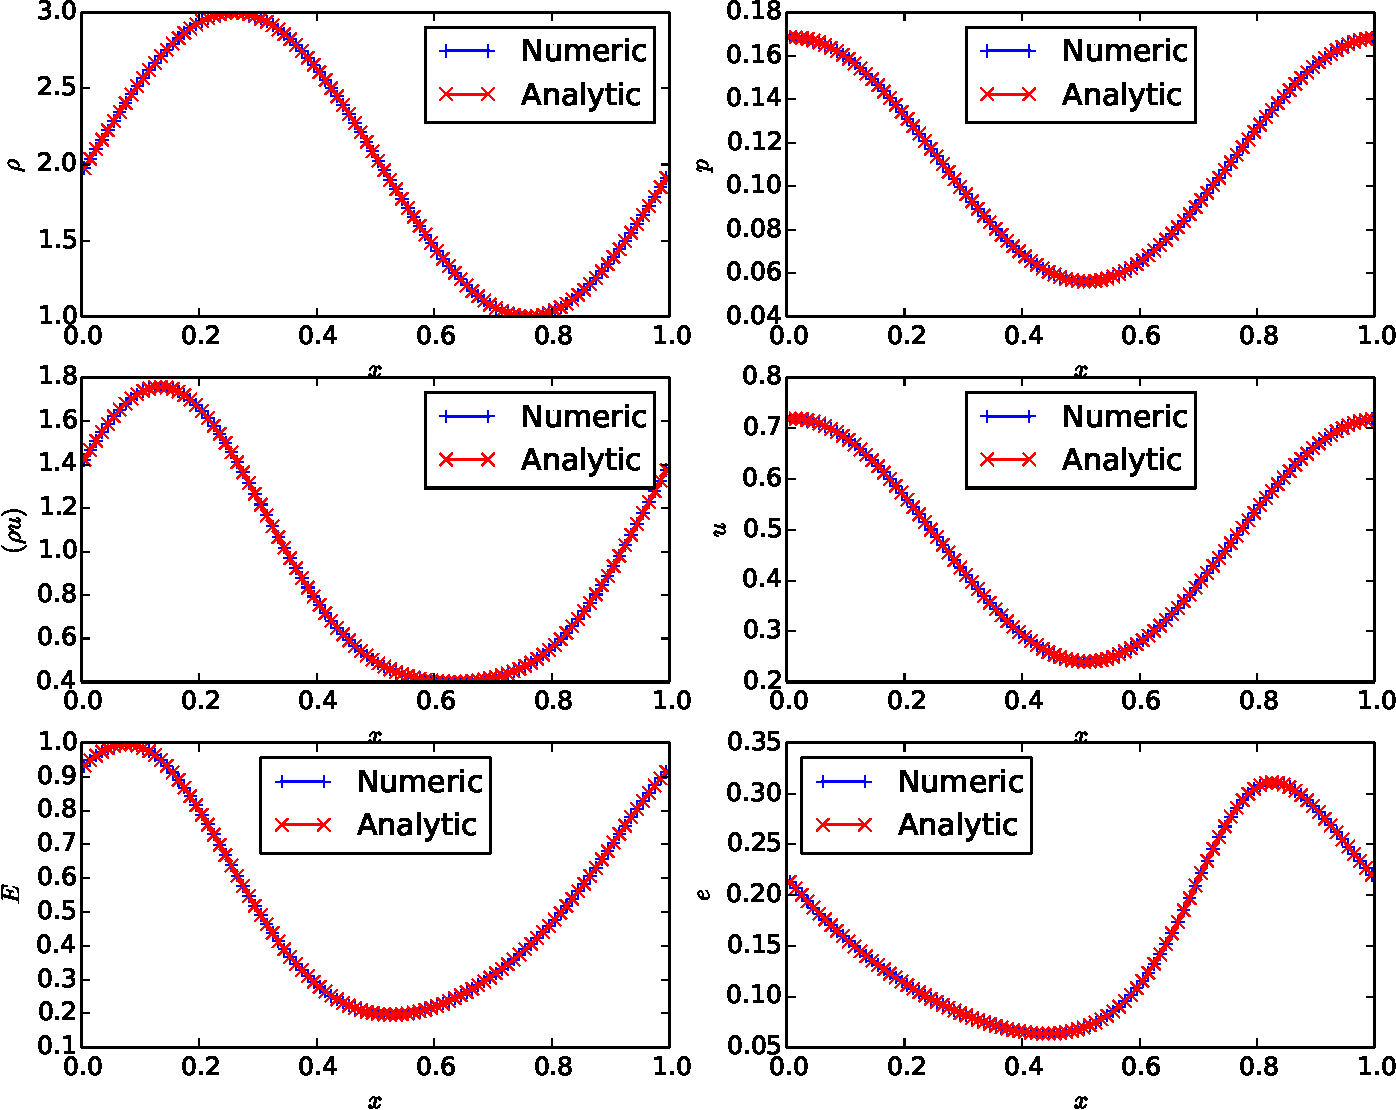
\includegraphics[width=\textwidth]{figures/MMS_diffusion_limit_solution.pdf}
   \caption{Hydrodynamic solution for the equilibrium diffusion limit MMS problem}
   \label{fig:MMS_diffusion_limit_solution}
\end{figure}

\begin{figure}[ht]
   \centering
   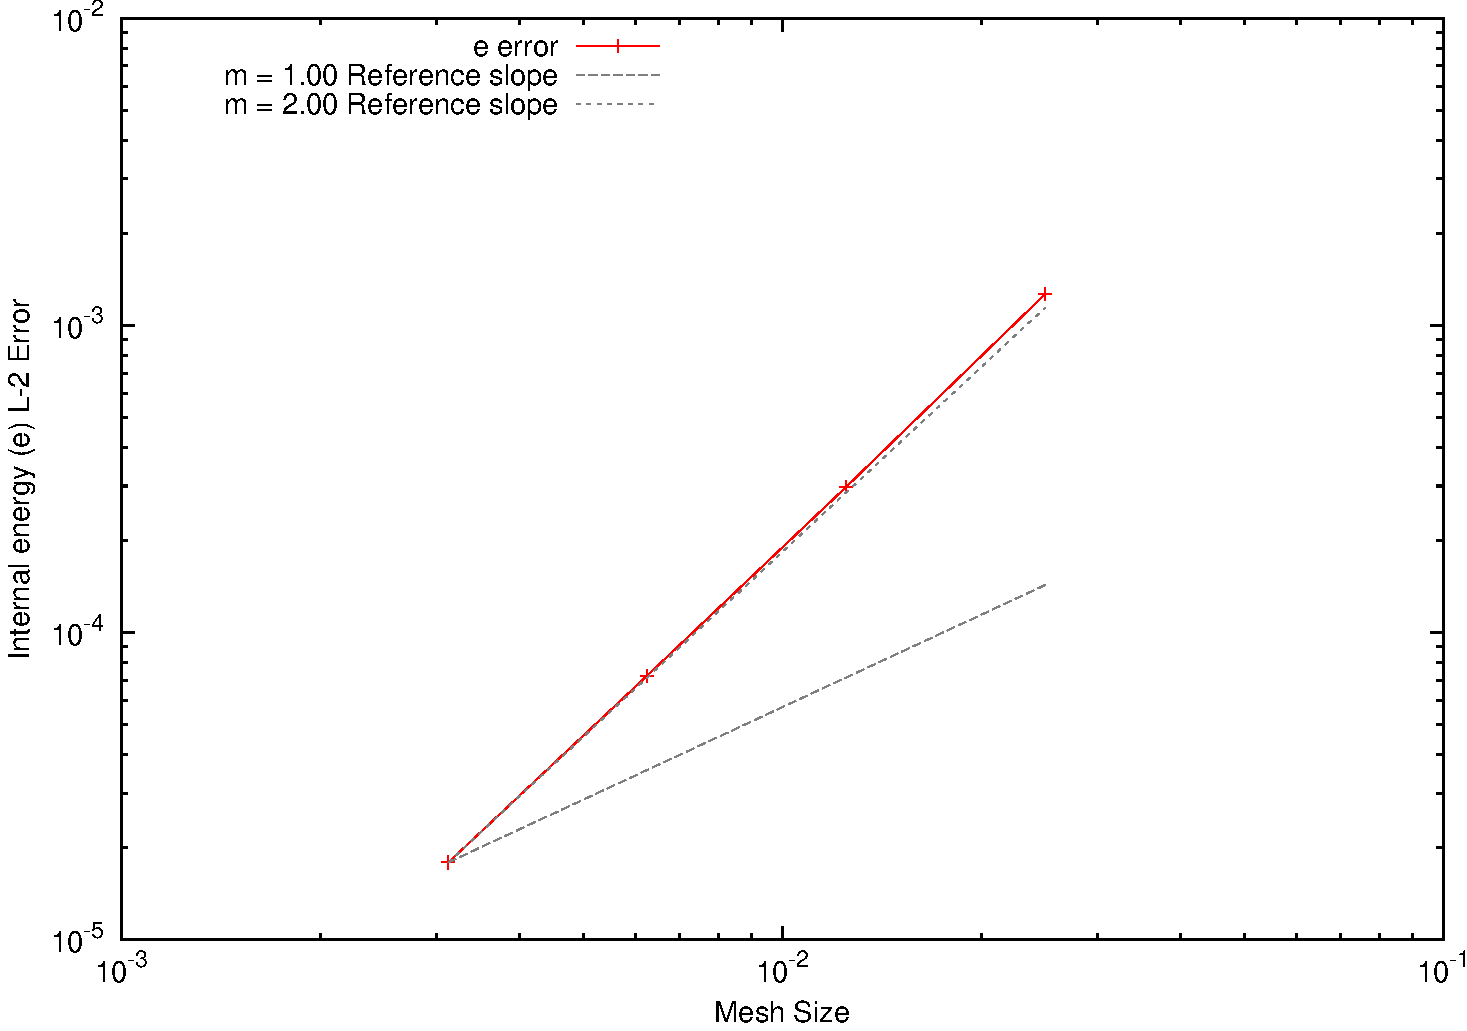
\includegraphics[width=\textwidth]{figures/MMS_diffusion_limit_convergence.pdf}
   \caption{Convergence of internal energy for the equilibrium diffusion limit MMS problem}
   \label{fig:MMS_diffusion_limit_convergence}
\end{figure}

The second MMS problem corresponds to the streaming limit, in which the radiation
and hydrodynamics are weakly coupled due to the high radiation energy propagation
speed relative to the fluid speed. For this problem, the following MMS solutions
are chosen:

%\begin{subequations}
%\end{subequations}

\subsection{Radiation-Hydrodyamics Shocks}
%-------------------------------------------------------------------------------
A Mach 2 radiative shock problem was taken from \cite{edwardsthesis}.
The material properties are uniform and are given in Table
\ref{tab:mach2_shock_material}. Initial conditions in the pre-shock
and post-shock regions are given in Table \ref{tab:mach2_shock_IC}.
Figure \ref{fig:mach2_shock_T} shows the numerical solution computed
with 300 cells and a CFL of 0.6, using the van Leer slope limiter;
the comparison to the reference solution shows excellent agreement.

\begin{table}[ht]
  \centering
  \caption{Material property values for the Mach 2 radiative shock problem}
  \label{tab:mach2_shock_material}
  \begin{tabular}{l l}\hline
    \emph{Parameter} & \emph{Value}\\\hline
    $\sigma_a$ & 390.71164263502112\\
    $\sigma_t$ & 853.14410158161809\\
    $c_v$      & 0.12348\\\hline
  \end{tabular}
\end{table}

\begin{table}[ht]
  \centering
  \caption{Initial condition values for the Mach 2 radiative shock problem}
  \label{tab:mach2_shock_IC}
  \begin{tabular}{l l l}\hline
    \emph{Parameter} & \emph{Pre-shock Value} & \emph{Post-shock Value}\\\hline
    $\rho$           & 1                      & 2.2860748989303659\\
    $u$              & 0.23426480742954117    & 0.10247468599526272\\
    $E$              & 3.9788000000000004e-2  & 7.0649692950433357e-2\\
    $\E$             & 1.3720000000000002e-6  & 2.5560936967521927e-5\\
    $\F$             & 0                      & 0\\\hline
  \end{tabular}
\end{table}

\begin{figure}[ht]
   \centering
   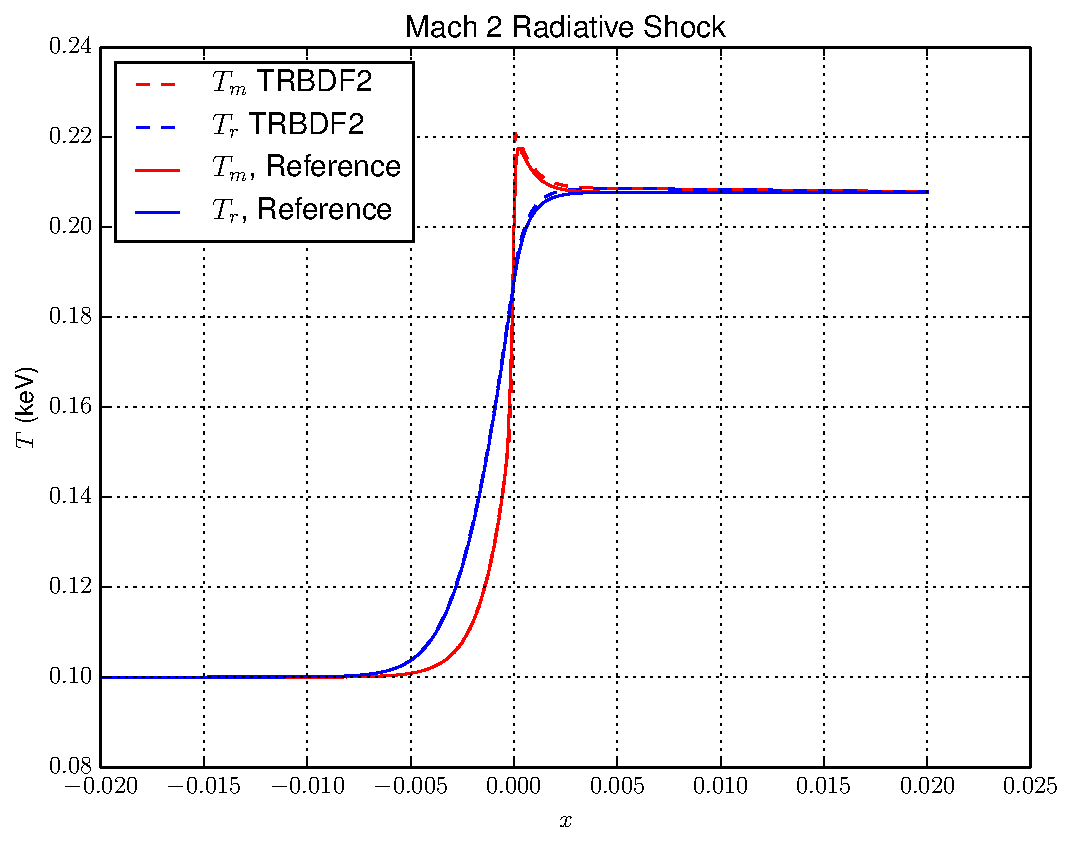
\includegraphics[width=\textwidth]{figures/mach2_shock_T.pdf}
   \caption{Comparison of Mach 2 radiative shock solution to reference solution}
   \label{fig:mach2_shock_T}
\end{figure}



\section{References}
\bibliographystyle{bibstyle}
\bibliography{references}

\end{document}
